\chapter{Non-linear power spectra: Resummation for Horndeski models \label{chap:nonlinear}} % Main chapter title

 % For referencing the chapter elsewhere, use \ref{Chapter1} 

%----------------------------------------------------------------------------------------


%----------------------------------------------------------------------------------------

As we have seen in previous chapters, non-linearities contain very valuable information
on the parameters of the model governing the evolution of structures in the Universe.
A proper understanding of the non-linear regime of structure formation is of fundamental 
importance in order to be able to analyze future observations of galaxy surveys and 
to discriminate between different cosmological scenarios.

Since this has become such an important issue in the last few years, there has been 
substantial progress in the theoretical and numerical
treatment of non-linearities for cosmological structure formation. 
From very advanced N-body simulations
\mcite{Springel, Illustris, Teyssier, Baldi, Winther, COLA, gevolution}, to
comprehensive semi-analytical methods \mcite{Halofit, HMcode, Halo model, Cosmic Emu, 
PkAnn} and complex resummation and renormalization methods \mcite{RPT, eRPT,
2LPT, regPT, gRPT, tSPT, EFTofLSS, TRG, Coarse}. There has also been a great advance in
new statistical tools for analyzing non-linear, non-Gaussian cosmic structures, see
\mcite{Large deviation, Minkowski functionals, Bispectrum, Separate Universe, 
analytic Covariance}.

Here we apply for the first time the Eikonal Renormalized Perturbation Theory (eRPT) developed
by \cite{anselmi_nonlinear_2012}, \mcite{Pietroni, recent, 2016} to the 
case of Horndeski models which were treated in \cref{sub:EFT-of-DE}.
In order to do so, we will take some simplifying assumptions like the quasistatic limit and
some specific variations of the $\mu$ and $\eta$ functions, previously
defined in \crefrange{eq:mu_def}{eq:eta_def}.

The chapter is organized as follows:
In \cref{sec:nonlinear-fluid} we start from the Vlasov-Poisson
system and write down the fluid equations for a non-relativistic matter component.
Then we show, using the quasistatic limit, which modified gravity functions we are going to 
take into account from Horndeski's theory.
In \cref{sec:field-notation} we write down the continuity, Euler and Poisson equations in a unified
field notation, which is the basis of our resummation method.
Finally in \cref{sec:linear propagator} and \cref{sec:The-Evolution-Equation} we will detail
the formalism of the eRPT method, computing the propagator 
and the evolution equation for the power spectrum, but mostly focusing on how it is modified in the Horndeski case. 
At the end of the chapter in \cref{sec:Computational} we make a short excursion through
computational techniques, like N-body simulations and semi-analytical methods, which
will be of importance for discussing this and the next chapter.

The equations, the results and most of the text of this chapter are based on a paper in preparation together with
Dr. Massimo Pietroni and Dr. Valeria Pettorino.


\section{Growth of perturbations for a Dark Matter component \label{sec:DM-growth}}

Before dealing with non-linear perturbation equations in modified gravity,
let us review the derivation of the evolution of the growth factor 
for a single Cold Dark Matter (CDM) component in linear theory.
This will help us introduce some quantities and 
relations that we will make use of in the next sections.
We will introduce the quasistatic approximation and 
then we will find a simple analytic formula for the growth factor $D_{+}(a)$
of CDM perturbations which will be useful later on. We will make use of the 
linearized Einstein equations  in the conformal Newtonian gauge, introduced in \cref{chap:DE-MG-Overview}, where we
follow the sign and naming conventions of the seminal work by \cite{MaBertschinger}.

If we transform \cref{eq:deltadot-general} and \cref{eq:thetadot-general} to
Fourier space, we obtain in the 
case of CDM which has a very simple equation of state $w=0$ and vanishing 
sound of speed and anisotropic velocity dispersion $c_s^2 = \sigma =0$:
\beeqal$
\dot{\delta}(\tau,\vk k) & =-\theta(\tau,\vk k)+3\dot\Phi(\tau,\vk k)  \label{eq:deltadot-CDM} \quad,\\
\dot{\theta}(\tau,\vk k) & =-\curH \theta(\tau,\vk k) + k^{2}\Psi(\tau,\vk k) 
\label{eq:thetadot-CDM} \quad,
$
where $\tau$ is the conformal time $\dx{}{\tau} = \dx{}{t}/a$ and an overdot 
represents a derivative with respect to $\tau$.

Derivating the first of the above equations with respect to $\tau$
and eliminating $\dot{\theta}$ and $\theta$ using both equations,
one obtains the second order differential equation for the density
contrast: 
\beeqc$\label{eq:deltadotdot}
\ddot{\delta} + \curH\dot{\delta} = 3 \curH \dot{\Phi} + 3\ddot{\Phi} -k^2\Psi  
$
for simplicity, we have dropped the arguments of the scale and time dependent functions.

At this stage we introduce the quasistatic (QS) approximation. In this approximation,
the first and second derivatives of the gravitational potential
$\Phi$ are taken to be negligible compared to the spatial gradients of $\Psi$. 
This is justified since the potentials vary only at cosmological time scales
and we are focusing on evolutions of the perturbations at subhorizon scales, where
$aH/k \gg 1$.
Now we apply the QS limit and use the relativistic Poisson equation \ref{eq:relativistic-Poisson} to substitute the Laplacian of $\Psi$ with a source term 
that depends on $\delta$:
\beeqp$ \label{eq:deltadotdot-sourced-tau}
\ddot \delta + \curH \dot\delta  = 4 \pi G a^2 \bar{\rho}_m  \delta 
$
In order to solve this equation, it is easier if we first transform 
our time variable to the scale factor $a$. To do so, we can define some transformations between conformal time and the scale factor:
\beeqal$
\curH &= \frac{\dot a }{a} = a \frac{\dd a}{\dd t} = a H \\
\dot \curH &=  \frac{\ddot a}{a} - \curH^2 \\
\frac{\dd{}}{\dd \tau} &= a^2 H \frac{\dd{}}{\dd a} \quad,
$
furthermore, from \cref{eq:Friedmann-1st} and \cref{eq:H-of-z-lcdm},
we can find the relation:
\beeqal$
\frac{4 \pi G}{H^2(a)} \rho_{m}(a) &= \frac{3}{2} \Omega_m (a) \quad,\\
\intertext{where, }
\Omega_m (a) = \frac{H_0^2 \Omega_{m,0} a^{-3}}{H^2 (a)} \quad.
$
Finally the transformed equation for $\delta$ has the form:
\beeqp$ \label{eq:deltaprimeprime}
\delta'' + \left( \frac{3}{a} + \frac{H'}{H} \right) \delta' = \frac{3}{2} 
\frac{\Omega_m (a)}{a^2} \,\delta 
$
This second order differential equation has two solutions: a decaying one, $D_{-}(a)$
and a growing one $D_{+}(a)$.
The decaying solution is $\delta \propto H$ and it can be shown easily by inspection
in the
matter dominated case where all the energy is non-relativistic matter (see \mcite{Dodelson book}). In that case,
$H \propto a^{-3/2}$ and all terms scale as $a^{-7/2}$, so that passing all terms to the 
left hand side, the coefficients 
$\{\frac{15}{4}, -\frac{9}{4} , -\frac{3}{2}\}$ indeed cancel out.
It can be shown that this decaying solution is satisfied even if $H$ contains
other energy components.
This can be done with the interesting relation between derivatives of $H$
and the matter species density fraction:
\beeqalsp$
\frac{H''(a)}{H(a)}+\frac{H'(a) \left(a H'(a)+3 H(a)\right)}{a H(a)^2} &= \\
   & \frac{3 H_0^2 \left(\Omega _{m,0}+\left(w_{\text{DE}}+1\right) \left(3 w_{\text{DE}}+1\right) \Omega _{\text{DE}} a^{-3 w_{\text{DE}}}\right)}{2 a^5 H^2} \quad,
$
where for generality, we have taken a \emph{wCDM cosmology}, with Hubble function:
\beeqc$\label{eq:Hprime-weff}
H^2 = H_0^2 \left( \Omega _{m,0} a^{-3}+\Omega _{\text{DE}} a^{-3
	\left(w_{\text{DE}}+1\right)}\right)
$
and Dark Energy equation of state $w_{\rm DE}$. With $w_{\rm DE}=-1$,
one can readily transform the r.h.s. of \cref{eq:deltaprimeprime}
and prove the validity of the decaying solution.

The growing mode of \cref{eq:deltaprimeprime} can be found by trying the 
Ansatz $u = \delta/H$ and by using the relation above \cref{eq:Hprime-weff},
between matter density and derivatives of $H$, we can find the evolution equation for 
$u$:
\beeqp$
u'' + 3 \left[ \frac{H'}{H} + \frac{1}{a} \right]u' = 0
$
Since there are no terms proportional to $u$,
this can be expressed as a first order equation of $v \equiv u'$:
\beeqal$
v' &= - 3 \left[ \frac{H'}{H} + \frac{1}{a} \right] v \nonumber\\
\ln v &= -3 \ln \left( a H \right) \nonumber \\
v &\propto (aH)^{-3} \quad .
$
This can be further integrated to find the growing mode, $D_{+}(a) \equiv \delta(a) 
 = u(a)H(a)$ as the integral:
\beeqc$ \label{eq:Dplus-Integral}
D_{+}(a)  = \frac{5 \Omega_{m,0}}{2 a_{\rm ini}} \frac{H(a)}{H_0} \int_{0}^{a} 
\frac{\dd{\tilde{a}}}{(\tilde a H(\tilde a)/H_0)^3}  
$
where the proportionality constant has been obtained by enforcing
$D_{+} = a$ at early matter-dominated times, when $H = H_0 \Omega_{m,0}^{1/2} a^{-3/2}$, 
see \mcite{Dodelson book} and $a_{\rm ini}$ is the scale factor at which
the initial condition $\Omega_{m}(a_{\rm ini}) = 1$, has been set. In this
way, \cref{eq:Dplus-Integral} matches exactly the numerical solution
of \cref{eq:deltaprimeprime}.

\begin{figure}[tbph]
	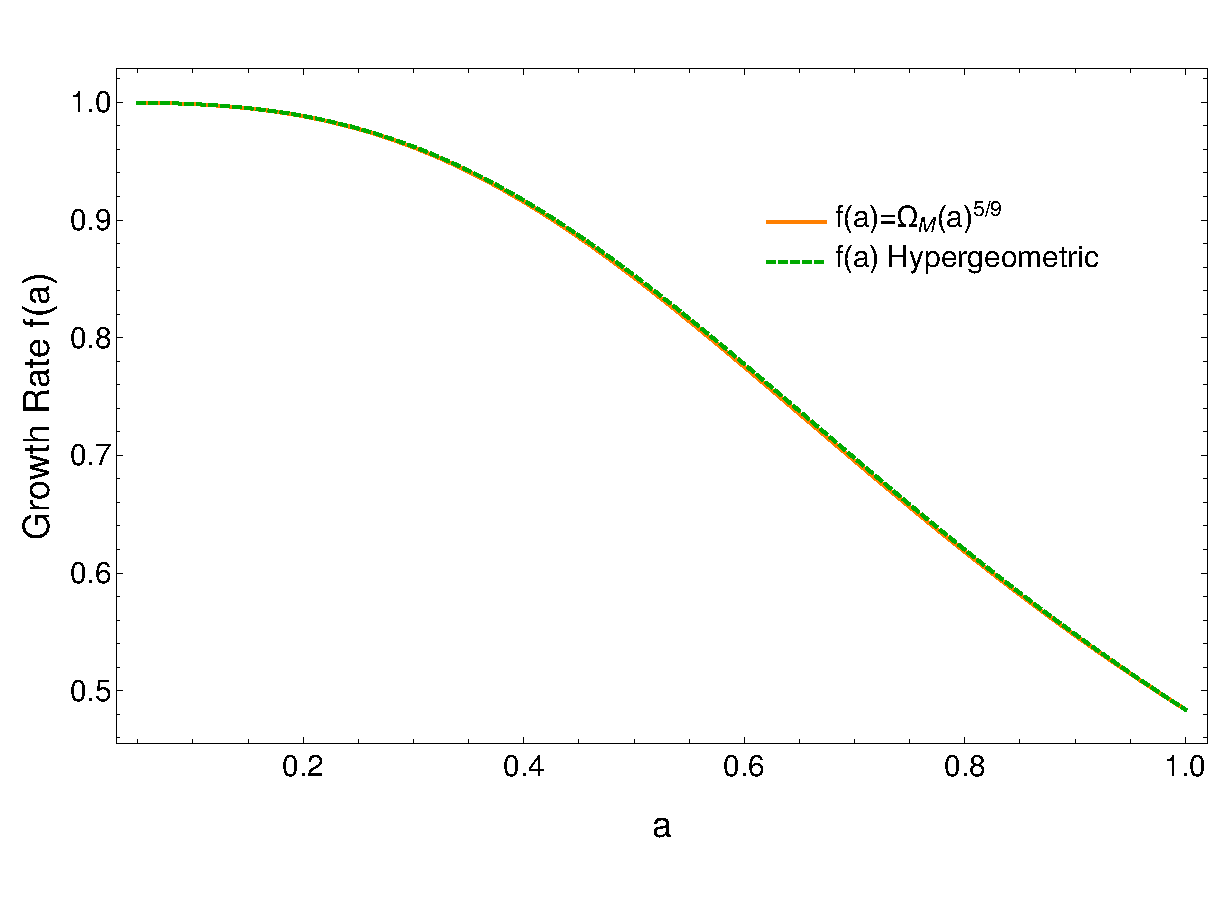
\includegraphics[width=0.47\linewidth]{Figures/fGrowthRate-ofa-Approx-vs-ExactHyper}
	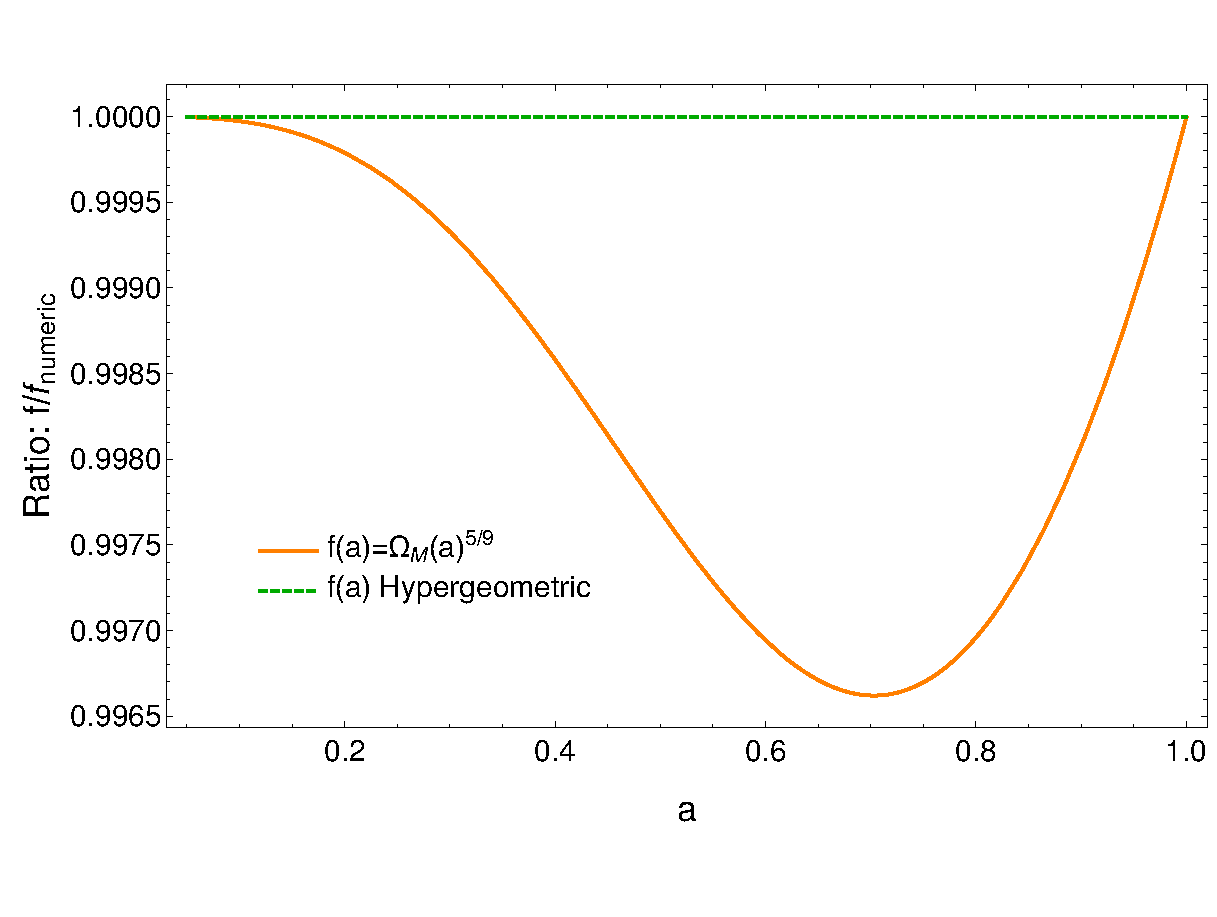
\includegraphics[width=0.47\linewidth]{Figures/fGrowthRate-Ratio-ofa-Approx-vs-ExactHyper-RatioToNumeric}
	\caption[Growth rate comparison for CDM]{
	\textbf{Left:} growth rate function $f(a)$, calculated by two different methods. In orange, the $\Omega^\gamma$-approximation, with $\gamma=5/9$, while
	in green the exact analytical solution from \cref{eq:Dplus-Hyper}.
    \textbf{Right:} Ratio of each of the two methods to the numerical solution of \cref{eq:fgrowth-of-N}, same coloring as before. The exact and numerical solution
agree exactly, while the $\gamma$-approximation is fine at the per mille level.}
	\label{fig:fgrowthrate-ofa-approx-vs-exacthyper}
\end{figure}



Usually, this integral in this form can only be expressed analytically for
an open Universe without Dark Energy (see \mcite{Dodelson book}).
However, by doing a further transformation into e-folding time: $ N \equiv \ln a$,
we can find a closed analytical expression
for the late-time $\lcdm$ scenario, with matter and a cosmological constant.
In this variable, the Hubble function looks like:
\beeqc$
H(N) = H_0 \sqrt{\Omega_{m,0} \exp{(-3 N)} + \Omega_{\Lambda,0} }
$
while the integral of \cref{eq:Dplus-Integral} transforms to:
\beeqp$\label{eq:Dplus-Nfolding-Integral}
D_{+}(N)  = \frac{5 \Omega_{m,0}}{2 a_{\rm ini}} H_0^2 H(a) \int_{-\infty}^{N} 
\frac{e^{-2 \tilde N} \dd{\tilde{N}}}{ H^3(\tilde N)}
$
It turns out that \cref{eq:Dplus-Nfolding-Integral} has a closed analytical
solution in the case of a cosmological constant and a total matter component.
It can be expressed in terms of Hypergeometric functions as:
\beeqp$\label{eq:Dplus-Hyper}
D_{+}(N) = \frac{1}{a_{\rm ini}} e^{N} \, _2F_1\left(\frac{1}{3},1;\frac{11}{6};-\frac{e^{3 N} \Omega_{\Lambda,0}}{ \Omega_{m,0} } \right)
$
The growth rate which is defined as:
\beeqc$
f(a) = \frac{\dd{\,\ln} D_{+}(a)}{\dd \ln a} 
$
and it is usually approximated as $f(a)=\Omega^\gamma (a)$,
with $\gamma \approxeq 5/9$, 
can also be expressed in terms of Hypergeometric functions, as:
\beeqp$\label{eq:fgrowth-of-N}
f(N) = 1-\frac{6 e^{3 N} \Omega _{\Lambda ,0} \,\; _2F_1\left(\frac{4}{3},2;\frac{17}{6};-\frac{e^{3 N} \Omega _{\Lambda ,0}}{\Omega _{m,0}}\right)}{11 \Omega _{m,0} \;\, _2F_1\left(\frac{1}{3},1;\frac{11}{6};-\frac{e^{3 N} \Omega_{\Lambda ,0}}{\Omega _{m,0}}\right)}
$
It can be shown that $f(N)$ satisfies exactly the growth rate equation, which can be derived
from \cref{eq:deltaprimeprime} and we express here in terms of the e-folding time
$N = \ln a$:
\beeqp$\label{eq:f-of-N-diffeq}
 \totder{f}{N} + f^2 + \left( 2 + \totder{\,\ln H}{N} \right) f = \frac{3}{2} \Omega_m
$
In \cref{fig:fgrowthrate-ofa-approx-vs-exacthyper} we show the result
for the formulas presented above. In the left panel,
we show $f(a)$ for the $\gamma$ approximation (orange solid line) compared
to the exact $f(a)$ solution of \cref{eq:fgrowth-of-N}. The difference is almost unnoticeable
by eye. Notice how at early times, when most of the energy of the Universe
consisted on non-relativistic matter, the growth rate is equal to unity and it 
decreases due to the later dominance of Dark Energy.
In the right panel of \cref{fig:fgrowthrate-ofa-approx-vs-exacthyper},
we plot the ratio between the $\gamma$-approximation and the numerical solution
of \cref{eq:fgrowth-of-N} in orange solid lines,
while in dashed green we plot the ratio of the exact solution to the numerical one.
The latter agrees exactly, while the $\gamma$-approximation is accurate at the per mille level.

\section{The non-linear fluid equations \label{sec:nonlinear-fluid}}

In order to study large scale structure (LSS) formation we will treat the Dark
Matter distribution as a perfect fluid of collisionless particles
coupled to gravity. These particles, with positions $\vk x$, mass
$m$ and momenta $\vk p$, are described by the Vlasov equation
in phase-space, with the phase space density $f(\vk x, \vk p, \tau)$
:
\beeqp$
\totder{f}{\tau} = \parder{f}{\tau} + \frac{\vk p}{m a} \nabla f -
a m \nabla \Psi \cdot \parder{f}{\vk p}
$
This equation together with the Poisson equation \cref{eq:Newtonian-Poisson},
form the Vlasov-Poisson system (see \cite{bernardeau_large-scale_2001}).
Since we are interested in the evolution in time of the spatial distribution,
we can take momentum moments of the Vlasov equation. This will yield
an infinite hierarchy of coupled differential equations, where the zeroth-moment
of the phase-space distribution ($\rho$) is coupled to the first-moment ($\vk u$),
the first-moment to the second $\sigma_{ij}$ and so on (see \cite{bernardeau_large-scale_2001}).
For our purposes we will neglect the anisotropic stress tensor $\sigma_{ij}$,
which describe velocity dispersion and anisotropic pressure.
and so on.
This is the so-called \emph{single stream approximation} and is one of
the main limitations of Eulerian perturbation theory, since the theory
breaks down as soon as shell crossing and multi-streaming start being
important.

From the first two momentum-moments of the Vlasov equation, giving rise
to the continuity and Euler equations, together 
with the Poisson equation, we can find the fluid equations of the system, 
where we will add from the start two general terms $\mathcal{A} (\vk x,\tau)$
and $\mathcal{B} (\vk x,\tau)$ in real space, which account for modifications
of gravity either in the Einstein or Jordan frames (see \cite{pietroni_flowing_2008}):
\beeqal$ 
\dot{\delta}(\vk x,\tau) & +\nabla\cdot\left[\left(1+\delta(\vk x,\tau)\right)\vk v (\vk x,\tau)\right]=0\label{eq:continuity}\\
\begin{split}
\dot{\vk v} (\vk x,\tau) & +\curH \left( \vk v (\vk x,\tau) + \left[\mathcal{A} (\vk x,\tau)\vk v (\vk x,\tau)\right] \right) \\
                         & + \left(\vk v (\vk x,\tau) \cdot\nabla\right)\vk v (\vk x,\tau)=-\nabla\Psi (\vk x,\tau)   \label{eq:euler}
\end{split}\\
\nabla^{2}\Psi(\vk x,\tau) & =\frac{3}{2}\curH^{2}(\tau)\Omega_{m}(\tau)\left(\delta (\vk x,\tau)+\left[\mathcal{B}(\vk x,\tau) \delta (\vk x,\tau)\right]\right)\label{eq:MG-poisson-fluid}
$
Here, as usual in our notation, $\tau$ is the conformal time, and an overdot represents a derivative with respect to $\tau$. The
symbols $\delta_{c}(\vk x,\tau)$ and $\vk v(\vk x,\tau)$
are respectively the matter density contrast and the peculiar velocity. $\Psi(\vk x,\tau)$ is
the $00$-gravitational potential and the functions $\mathcal{A}(\vk x,\tau)$
and $\mathcal{B}(\vk x,\tau)$ are general functions of space and
time that parameterize different cosmologies, for example when particles' geodesics
are modified, or when there is an extra ``fifth-force`` acting between Dark Matter particles.
This can happen
due to couplings with a scalar field or more general modifications
of gravity, see \cref{chap:DE-MG-Overview} for more details.
However, in the Jordan
frame, where Horndeski's theory is formulated, the Euler equation is
not modified and there is only a space-time dependent modification
to the Poisson equation, which will be connected to the scale-time dependent
function $\mu(k,t)$, defined below and used extensively in the previous \cref{chap:lin-nonlin-MG-forecasts}.
Within this chapter,  $\Omega_{m}(\tau)$
is the function representing the cold dark matter (CDM) density of the Universe.
For simplicity, we will neglect baryonic matter and neutrinos. 

In the following, we will stay within the quasi-static
limit, i.e restrict to scales much smaller than the cosmological horizon
($k/aH\gg1$) and well inside the Jeans length of the scalar field
$c_{s}k\gg1$, so that terms containing $k$ dominate over terms containing
time derivatives. So that \cref{eq:deltadotdot-sourced-tau} is the equation
governing the evolution of matter perturbations.


For general modified gravity theories, the deviation
of the gravitational potentials from General Relativity,
can be parameterized with two arbitrary functions
of scale and time: $\mu(k,a)$ and $\eta(k,a)$,
as was explained in \cref{chap:DE-MG-Overview}, \cref{sub:parameterizing-MG}.
However, in the quasistatic limit for Horndeski theories, these two functions have a specific form, given by \mcite{amendola, observables, bellini}: 
\begin{equation}
\mu(k,a)\equiv-\frac{2k^{2}\Psi}{3\Omega_{m}\delta_{m}}=h_{1}\left(\frac{1+(k/k_{*})^{2}h_{5}}{1+(k/k_{*})^{2}h_{3}}\right)\label{eq:mufunc}
\end{equation}
where $h_{1},h_{3},h_{5}$ are functions of time only. A similar expression,
with different time dependent coefficients $h_{2},h_{4}$, holds for
the gravitational slip $\eta$: 
\begin{equation}
\eta(k,a)\equiv-\frac{\Phi}{\Psi}=h_{2}\left(\frac{1+(k/k_{*})^{2}h_{4}}{1+(k/k_{*})^{2}h_{5}}\right)\,.\label{eq:etaFunc}
\end{equation}
For the remainder of this chapter, we will consider all $h_{i}$ functions as constants in order to simplify our computations and to show the main effects of MG, without specifying
a model. The scale $k_{*}$ is an arbitrary pivot scale, which can be chosen accordingly.
As it can be seen from  \cref{eq:mufunc} and \cref{eq:etaFunc},
the functions $h_{5}$ and $h_{3}$ are degenerate as well as $h_{4}$
and $h_{5}$. The $\Lambda\textrm{CDM}$ case is recovered when $\mu=\eta=1$, which
implies $h_{5}=h_{4}=h_{3}$ and an amplitude $h_{1}=h_{2}=1$.

Since we are in the QS limit, the only MG function entering the perturbation equations
is $mu(a,k)$. The function $\eta(a,k)$ could enter the equations
if we would not neglect the derivatives of the gravitational potential $\Phi$, as 
was shown in \cref{chap:lin-nonlin-MG-forecasts}.
In the following we will only consider the scale-dependence of $\mu$, therefore $\mu(k,a)=\mu(k)$ (although perturbations require
two functions of time and scale to fully specify the model). In particular,
we will test the following cases: 
\begin{enumerate} \label{enum:enumeration-cases}
	\item Scale independent $\mu$ with modified amplitude: $h_{5}=h_{3}$ and
	$h_{1}>1$ or $h_{1}<1$. 
	\item Scale dependent $\mu$ with unity amplitude: $h_{1}=1$ and $h_{5}>h_{3}$
	or $h_{5}<h_{3}$. 
	\item Scale dependent $\mu$ with modified amplitude: $h_{1}\neq1$ and
	$h_{5}>h_{3}\mbox{ or }h_{5}<h_{3}$. 
\end{enumerate}
An example of these $\mu(k)$ functions is shown in \cref{fig:Mu(k)function}, where we show the 
function $\mu(k)$ for three different cases. The solid blue line stands for case 1, in which only the amplitude of
$\mu$ changes, but there is no scale dependence. The orange dashed line in this figure, stands for case 2, 
in which the amplitude is unity at large scales and there is a $k$-dependence at smaller scales. 
Finally, in dot-dashed-green, we show case 3 in which both the amplitude and the scale-dependence deviate from standard GR.
\begin{figure}[htbp]
	\centering
	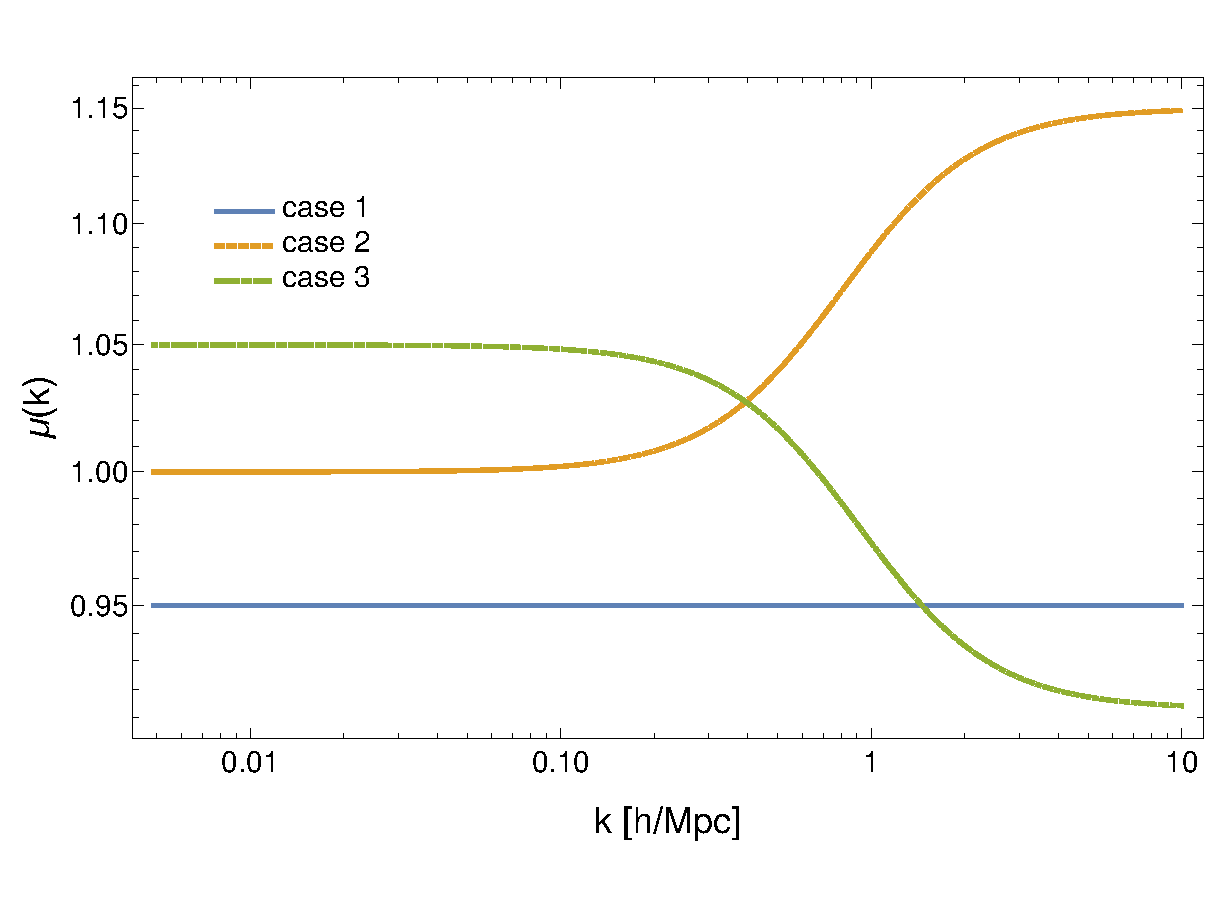
\includegraphics[width=0.75\linewidth]{Chapters/resummation-plots/mu-of-k-plots-3cases.pdf}
	\caption[MG function $\mu(k)$]{Function $\mu(k)$ for three different cases specified in the text. The solid blue line stands for case 1, in which only the amplitude of
	$\mu$ changes, but there is no scale dependence. The orange dashed line is case 2, 
in which the amplitude is unity at large scales and there is a $k$-dependence at smaller scales. In dot-dashed-green, we show case 3 in which both the amplitude and the scale-dependence deviate from standard GR.}
	\label{fig:Mu(k)function}
\end{figure}

%
%In logarithmic space $\mu(k)$ is very close to a step function, as
%shown in figure \ref{fig:Y(k)-function}, so that we will only use
%values for the $h_{i}$ in which the difference of the minimum and
%the maximum is of the order of 15\%, since otherwise we would impose
%a rather unrealistic structure formation.
%\section{Standard perturbation theory and higher orders}
%\begin{itemize}
%\item Vlasov-Poisson system
%\item System of equations in Fourier space
%\item Velocity divergence and vorticity
%\item Stress tensor and higher order hierarchy terms
%\item Field variable doublet and 1-loop expansion
%\end{itemize}



\section{The field notation\label{sec:The-field-notation}}


We can express \crefrange{eq:continuity}{eq:MG-poisson-fluid} in a compact
form, known as the field notation, which was introduced in the literature of
standard perturbation theory (SPT) and renormalized
perturbation theory (RPT) (see \cite{bernardeau_large-scale_2001,crocce_renormalized_2005,pietroni_flowing_2008}). 
To do so, we will transform \crefrange{eq:continuity}{eq:MG-poisson-fluid} into Fourier space.
In linear theory, this is a straightforward computation,
since partial derivatives transform into $\partial \rightarrow ik$.
However, if we take into account the non-linear terms, these become convolutions
in Fourier space.
First we decompose the velocity such that:
\begin{equation}
\vk v(\vk k)=\vk v_{\theta}(\vk k)+\vk{v{}_{\omega}}(\vk k) \quad,
\end{equation}
where:
\begin{align*}
\vk k\cdot\vk{v_{\omega}}(\vk k) & =0\\
\vk k\times\vk{v_{\theta}}(\vk k) & =0
\end{align*}
According to linear theory the vorticity component $\vk{v{}_{\omega}}(\vk k)$
decays with the expansion of the Universe as $a^{-1}$, so if we assume
non-vortical initial conditions, we can neglect this term and look
only at the velocity divergence $\theta=i\vk k\cdot\vk v$, which
is now a scalar function. Inverting this last relation to get: $\vk v=-\frac{i\vk k}{k^{2}}\theta$,
allows us to perform the Fourier transforms explicitly:
\begin{align*}
\mathit{FT}\left\{ \nabla\cdot(\delta_{m}\vk v)\right\}  & =+i\vk k\int\d^{3}q\d^{3}p\delta_{D}(\vk p+\vk q-\vk k)\frac{-i\vk p}{p^{2}}\delta_{m}\ppt q\theta\ppt p\\
& =\int\d^{3}q\d^{3}p\delta_{D}(\vk k-\vk p-\vk q)\underbrace{\frac{\left(\vk p+\vk q\right)\cdot\vk p}{p^{2}}}_{\alpha(\vk p,\vk q)}\delta_{m}\ppt q\theta\ppt p
\end{align*}
\begin{align*}
\mathit{FT}\left\{ \nabla\cdot\left[\left(\vk v\cdot\nabla\right)\cdot\vk v\right]\right\}  & =i\vk k\cdot\int\d^{3}q\d^{3}p\delta_{D}(\vk q+\vk p-\vk k)\left(\frac{-i\vk q}{q^{2}}\cdot i\vk p\right)\frac{-i\vk p}{p^{2}}\theta\ppt q\theta\ppt p\\
& =\vk k\cdot\int\d^{3}q\d^{3}p\delta_{D}(\vk k-\vk q-\vk p)\left(\frac{\vk p\cdot\vk q}{p^{2}q^{2}}\right)\vk p\,\theta\ppt q\theta\ppt p\\
& =\int\d^{3}q\d^{3}p\delta_{D}(\vk k-\vk q-\vk p)\underbrace{\frac{(\vk p\cdot\vk q)^{2}\vk p\cdot\vk q}{2p^{2}q^{2}}}_{\beta(\vk q,\vk p)}\theta\ppt q\theta\ppt p
\end{align*}
where in the last step we used the symmetry between $\vk p$ and $\vk q$.
The terms marked with an underbrace, are the ones responsible for
the mode-mode coupling:
\begin{equation}
\alpha(\vk q,\vk p)=\frac{(\vk p+\vk q)\cdot\vk q}{q^{2}}=\alpha(-\vk q,-\vk p);\;\beta(\vk q,\vk p)=\frac{(\vk p+\vk q)^{2}\vk p\cdot\vk q}{2p^{2}q^{2}}=\beta(-\vk q,-\vk p)\label{eq:alpha-beta-func}
\end{equation}
Defining a field doublet $\varphi_a$, with index $a$ as: 
\begin{equation}
\vpa a\pkn=e^{-\eta}\colv{\delta_{m}\pkn}{-\theta\pkn/\curH} \quad,\label{eq:field-doublet}
\end{equation}
we obtain the Euler, continuity and Poisson equations in a compact form:
\begin{equation}\label{eq:field notation}
\partial_{\eta}\varphi_{a}(\vk k,\eta)=-\Omega_{ab}\pkn\varphi_{b}\pkn+e^{\eta}\gamma_{abc}(\vk k,\vk{-p},\vk{-q})\vpa b\ppn p\vpa c\ppn q \quad.
\end{equation}
In the above equation we have defined a new time variable which will prove to be very convenient for our calculations:
\beeqp$ 
\eta\equiv\ln\frac{a}{a_{in}}
$
The r.h.s. of  \cref{eq:field notation} contains two terms, the first one
corresponds to the ``linear`` evolution of perturbations, where the $\Omega_{ab}$
matrix encodes the cosmology dependence:
\begin{equation}\label{eq:general-Omega-Matrix}
\Omega_{ab}\pkn=\begin{pmatrix}1 & -1\\
-\frac{3}{2}\Omega_{m}(\eta)(1+\mathcal{B}\pkn) & 2+\frac{\curH'}{\curH}+\mathcal{A}\pkn
\end{pmatrix} \quad,
\end{equation}
where here the functions $\mathcal{B}\pkn$ and $\mathcal{A}\pkn$ are the Fourier space
transforms of the same functions defined in the Vlasov-Poisson system 
and encode possible modifications of gravity.
In Horndeski theories under the QS limit, we can identify:
\beeqal$
(1+\mathcal{B}\pkn) = \mu(\eta,k) \\
\mathcal{A}\pkn = 1 \quad.
$

On the r.h.s. of  \cref{eq:field notation}, the second term represents
all the nonlinearities in real space and therefore non-localities in Fourier space.
The $\gamma_{abc}$ functions
in this formalism can be understood as interaction vertices and its
only non-vanishing components are precisely given by the mode-mode
coupling functions $\alpha \textrm{ and } \beta$, defined in \cref{eq:alpha-beta-func} : 
\begin{align}
\gamma_{121}\pcq kpq & =\frac{1}{2}\delta_{D}\psq kpq\alpha(\vk p,\vk q) & \;\gamma_{121}\pcq kqp=\gamma_{112}\pcq kpq\label{eq:coupling-vertices}\\
\gamma_{222}\pcq kpq & =\delta_{D}\psq kpq\beta(\vk p,\vk q)\nonumber 
\end{align}
In this notation and throughout this work, an \emph{integration over} $\vk p,\vk q$
\emph{is understood} and $\vk k$ is always the ``external'' momentum.
The integral symbols will be added only if they are needed due to possible confusions
with the notation.

%\texttt{Due to mode-mode coupling, there is a loss of information about the
%initial conditions in the limit of high-k, since density perturbations
%get mixed \cite{crocce_memory_2006}. This has as a consequence that
%highly-nonlinear corrections to the power spectrum become cosmology-independent
%in a rough way.}



%Where we have the usual definitions: $\curH=aH,\; a\mbox{d}\tau=\mbox{d}t,\; a'=\frac{\mathrm{d}a}{\d\ln a}=a,\;\frac{\curH'}{\curH}=\frac{H'}{H}+1,$
%where $':=\frac{\d}{\d\ln a}$ and $N\equiv\ln a$ is what is typically
%called the e-foldings time.

%For details on how to go back to the usual fluid equations \ref{eq:continuity}-\ref{eq:poisson}
%in Fourier space starting from the field equation \ref{eq:field notation},
%see Appendix \ref{sec:Appendix-field-equations}.

Equation \ref{eq:field notation} is the starting point for all renormalization
and resummation methods, like the ones introduced by \cite{crocce_renormalized_2005,bernardeau_evolution_2013,bernardeau_constructing_2012,
	valageas_matter_2013,anselmi_nonlinear_2012,anselmi_next--leading_2010}.
The linear part can be easily solved and the function relating the
initial primordial density perturbations to the final one, is called
the linear propagator and will be studied in section \ref{sec:linear propagator}.
The nonlinear part, cannot be solved analytically, nor with a simple
numerical integration.
However, a perturbative approach using tools from Quantum Field Theory
can be used to regularize its divergences which are caused by the
fact that the density perturbations (which is at the same time the
perturbation variable) grows with time and increasing wave vector.
For this part we will use the resummation technique of \cite{anselmi_nonlinear_2012}
and this will be explained in detail in section \ref{sec:The-Evolution-Equation}.

Resumming and renormalizing perturbation theory can help in finding the evolution
of the nonlinear power spectrum at small scales and late times, but
even if we could calculate exactly its result at all loop orders,
there are still intrinsic limitations given by the starting equations
\ref{eq:continuity}-\ref{eq:poisson}. Apart from neglecting vorticity
in the later stages of evolution, the initial equations are derived
in the single-stream-approximation. This means that at a single point
in space, there can be only one velocity direction. This clearly breaks
down in the virialization regime and even before during late stages of structure formation. 
Resummation methods
can be extended and improved by including these other sources of density
power into the equations in an effective way, see the discussion in
\cite{manzotti_coarse_2014,pietroni_coarse-grained_2011} and recent
results in the effective field theory of large scale structures \cite{baumann_cosmological_2012,pajer_renormalization_2013,senatore_ir-resummed_2014,carrasco_effective_2012}.

In the following sections, we will show how to solve the linear part of
the fluid equations for a general time and scale-dependent growth (see \cref{sec:linear propagator})
and then we will use these results in \cref{sec:The-Evolution-Equation} to solve the evolution equation of the 
matter power spectrum, which will yield the non-linear evolution
of the density perturbations.


\section{The linear propagator \label{sec:linear propagator}}

As was explained above, in eqn. \ref{eq:field notation} the non-linearity
of the Vlasov-Poisson system of equations is fully encoded in the
vertex $\gamma_{abc}$ which represents the mode-mode coupling. Without
this term, we recover the linear equation:
\begin{equation}
\pet\vpa a\pkn=-\Omega_{ab}\pkn\vpa b\pkn \label{eq:linear-field}
\end{equation}
which is valid for a fully scale and time dependent $\Omega_{ab}$. 
The linear propagator is the function that connects the initial
density perturbations with the final ones, or in other words solves
the above equation (\ref{eq:linear-field}) (see \mcite{scoccimarro, pietroni}).
The linear propagator gives the linear
evolution of the field $\vpa a$:
\beeqc$ 
\vpa a\pkn=g_{ab}(\vk k,\eta,\eta')\vpa b\pkn
$
and it has to fulfill following properties:
\begin{align*}
\pet g_{ab}(\vk k,\eta,\eta') & =-\Omega_{ac}\pkn\cdot g_{cb}(\vk k,\eta,\eta')\\
\lim_{\eta'\rightarrow\eta}g_{ab}(\vk k,\eta,\eta') & =\mathbbm{1}_{ab}\\
g_{ab}(\vk k,\eta,\eta')\cdot g_{bc}(\vk k,\eta',\eta'') & =g_{ac}(\vk k,\eta,\eta'')
\end{align*}

\subsection{The linear propagator in the general case}

We can show that the linear propagator can be written in general for the scale and time 
dependent decaying ($-$) and growing ($+$) modes of the growth rate $f_{\pm}(\vk k,\eta)$ as:
\begin{equation}
\begin{aligned}g(\vk k,\eta,\eta') & =\Theta(\eta-\eta')\left[e^{-\int_{\eta'}^{\eta}(\Omega_{11}+\Omega_{12}f_{+})\d x}\begin{pmatrix}1 & 0\\
0 & \frac{f_{+}\pkn}{f_{+}(\vk k,\eta')}
\end{pmatrix}\mathrm{\mathbf{M}}{}^{+}(\vk k,\eta')\right.\\
& \left.+\, e^{-\int_{\eta'}^{\eta}(\Omega_{11}+\Omega_{12}f_{-})\d x}\begin{pmatrix}1 & 0\\
0 & \frac{f_{-}\pkn}{f_{-}(\vk k,\eta')}
\end{pmatrix}\mathrm{\mathbf{M}}{}^{-}(\vk k,\eta')\right]
\end{aligned} \quad ,
\label{eq:general-propagator}
\end{equation}
where $\mathbf{M}{^\pm}$ are projection operators which we will specify in the following
calculation (see \cite{pietroni_flowing_2008} for more details).

If the linear equation \cref{eq:linear-field}
has solutions of the form :
\beeqc$
\vpa{sol}\pkn=\begin{pmatrix}1\\
f\pkn
\end{pmatrix}\varphi\pkn
$
then we can find an equation that describes the evolution of the growth
of perturbations.
For the index $a=1$:
\begin{equation}
\pet\varphi=-\Omega_{11}\varphi-\Omega_{12}f\varphi=-(\Omega_{11}+\Omega_{12}f)\varphi\label{eq:linear-phi-eqn}
\end{equation}
For the index $a=2$:
\begin{align}
\pet(f\varphi) & =f\pet\varphi+\varphi\pet f=-\Omega_{21}\varphi-\Omega_{22}f\varphi\nonumber \\
\Rightarrow\pet f & =\Omega_{12}f^{2}+(\Omega_{11}-\Omega_{22})f-\Omega_{21}\label{eq:f-growth-rate}\\
\Rightarrow\pet f & =\Omega_{12}(f-\bar{f}_{+})(f-\bar{f}_{-})\label{eq:fgrowth-factorized-eqn}
\end{align}
Equation \ref{eq:f-growth-rate} is what we usually know as the growth
rate equation for $f=\d\ln D/\d\ln a$, being $D$ the growth factor
of density perturbations and in this general case it can have a time
and scale dependent solution. 
The zeros of \cref{eq:fgrowth-factorized-eqn} are given by:
\begin{equation}
\bar{f}_{\pm}\pkn=\frac{(\Omega_{22}-\Omega_{11})\mp\sqrt{(\Omega_{22}-\Omega_{11})^{2}+4\Omega_{21}\Omega_{12}}}{2\Omega_{12}}\label{eq:2.4}
\end{equation}
With these equations, we can find the solution of \cref{eq:linear-phi-eqn} and \cref{eq:fgrowth-factorized-eqn} as:
\begin{align*}
\varphi(\eta) & =e^{-\int_{\eta'}^{\eta}(\Omega_{11}+\Omega_{12}f)\d x}\varphi(\eta')\\
f(\eta)\varphi(\eta) & =e^{-\int_{\eta'}^{\eta}(\Omega_{21}+\Omega_{22}f)\d x}f(\eta')\varphi(\eta')\\
 & =e^{-\int_{\eta'}^{\eta}(\Omega_{11}+\Omega_{12}f)\d x}\varphi(\eta')f(\eta')\frac{f(\eta)}{f(\eta')}
\end{align*}
One can identify the basis solutions by setting their initial conditions
as:
\beeqc$
f_{\pm}^{in}=\bar{f}_{\pm}(\vk k,\eta_{i})
$
where $\eta_{i}$ is an initial time that can be set at high redshift
where the Universe is approximately Einstein-de Sitter (E-dS), therefore
matter dominated.

For E-dS, $\Omega_{m}=1$ we have very simple background quantities:
$\mathcal{H}'\backslash\mathcal{H}=-1/2-3w_{eff}/2=-1/2$, so that
the $\Omega_{ab}$ from equation \ref{eq:general-Omega-Matrix} is
simply:
\beeqc$ 
\Omega_{ab}=\begin{pmatrix}1 & -1\\
-\frac{3}{2} & \frac{3}{2}
\end{pmatrix}
$
which gives the following initial conditions for the growing $u$
and decaying $v$ modes:
\beeqal$ 
u_{a} &= \begin{pmatrix}1\\
f_{+}^{in}
\end{pmatrix}=\begin{pmatrix}1\\
1
\end{pmatrix} \\
v_{a} &= \begin{pmatrix}1\\
f_{-}^{in}
\end{pmatrix}=\begin{pmatrix}1\\
-\frac{3}{2}
\end{pmatrix}
$
The growing mode will be the mode of interest that we will use in
section \ref{sec:The-Evolution-Equation}, when we want to calculate
the evolution of the power spectrum.

The instantaneous projectors on the two basis solutions are defined
as:
\begin{align*}
\mathrm{\mathbf{M}}{}^{+}\pkn\begin{pmatrix}1\\
f_{+}\pkn
\end{pmatrix} & =\begin{pmatrix}1\\
f_{+}\pkn
\end{pmatrix}\\
\mathrm{\mathbf{M}}{}^{+}\pkn\begin{pmatrix}1\\
f_{-}\pkn
\end{pmatrix} & =0\\
\mathbf{\mathrm{\mathbf{M}}}^{-}\pkn\begin{pmatrix}1\\
f_{-}\pkn
\end{pmatrix} & =\begin{pmatrix}1\\
f_{-}\pkn
\end{pmatrix}\\
\mathrm{\mathbf{M}}^{-}\pkn\begin{pmatrix}1\\
f_{+}\pkn
\end{pmatrix} & =0
\end{align*}
In this case, the growing projector can be written explicitly by subtracting the
decaying projector from the unity matrix:
\beeqp$ 
\mathrm{\mathbf{M}}{}^{+}\pkn=\mathbb{1}-\mathrm{\mathbf{M}}{}^{-}\pkn=\frac{1}{f_{-}-f_{+}}\begin{pmatrix}f_{-} & -1\\
f_{-}f_{+} & -f_{+}
\end{pmatrix}
$
For the Einstein-de Sitter case, the projectors do not evolve in time,
since $u_{a}$ and $v_{a}$ are constant, and they are given by: 
\begin{align*}
\mathrm{\mathbf{M}}{}^{+} & =\frac{1}{5}\begin{pmatrix}3 & 2\\
3 & 2
\end{pmatrix}\\
\mathrm{\mathbf{M}}{}^{-} & =\frac{1}{5}\begin{pmatrix}2 & -2\\
-3 & 3
\end{pmatrix}
\end{align*}
In the E-dS case, since there is no $k$-dependence
in any quantity and the growing mode is constant, this would reduce to :
\beeqp$ 
g(\eta,\eta')=\Theta(\eta-\eta')\left[\frac{1}{5}\begin{pmatrix}3 & 2\\
3 & 2
\end{pmatrix}+\frac{1}{5}\begin{pmatrix}2 & -2\\
-3 & 3
\end{pmatrix}e^{-5/2(\eta-\eta')}\right]
$


\subsection{The linear propagator in the Horndeski case}

Using the same procedure as we employed for the general case, we will calculate the linear propagator
for the Horndeski case, in which the growth factor $D$ is scale
and time dependent. Then the linear propagator can be used to calculate
its fully nonlinear renormalized version, which then is a crucial
ingredient of the evolution equation in section \ref{sec:The-Evolution-Equation}.

Using \cref{eq:mufunc} as the modification of the Poisson equation
we can write the general $\Omega_{ab}$ matrix as:
\begin{equation}
\Omega_{ab}\pkn=\left(\begin{array}{cc}
1 & -1\\
-\frac{3}{2} \mu(k)\Omega_{m}(\eta) & \frac{\mathcal{H}'}{\mathcal{H}}+2
\end{array}\right)
\end{equation}
in this case, the initial conditions from \cref{eq:2.4} are: 
\begin{equation}
\begin{aligned}f_{-}^{in} & =-\frac{1}{2}(\Sigma+\omega)\\
f_{+}^{in} & =\frac{1}{2}(\Sigma-\omega)
\end{aligned}
\end{equation}
where $\omega=1+\frac{\curH'}{\curH}$
and $\Sigma=\sqrt{6Y\Omega_{m}+\omega^{2}}$ are quite general functions
of scale and time. Inserting this into \cref{eq:general-propagator},
one can find the most general form of the propagator for the Horndeski
theory. 
%However, this is not so practical, since we would have to
%solve for a scale and time dependent growth rate $f$ and evaluate
%the $\mathcal{H}$ function at each step.

For models which are close to $\Lambda\textrm{CDM}$, it is more convenient
to change the time variable from $\eta=\ln\frac{a}{a_{in}}$ to $\mychi=\ln\frac{D(\tau)}{D(\tau=\tau_{in})}$,
where $D(\tau)$ is the growth function usually written as the growing
solution of the linear density perturbation equation : $\delta(\tau)=D_{+}(\tau)\delta^{in}$.
%In our case, however, the time variable $\mychi$ would itself be
%scale dependent, since the growth rate equation in the Horndeski case
%is scale dependent, so that $\mathcal{X}(k)=\ln\frac{D(\tau,k)}{D(\tau=\tau_{in},k)}$.
%Using $\frac{\partial}{\partial\eta}=\frac{\d\ln D}{\d\ln a}\frac{\partial}{\partial\ln D}=f\frac{\partial}{\partial\mathcal{X}}$,
%we can rewrite eqns.\ref{eq:linear-phi-eqn}-\ref{eq:f-growth-rate}
%as (where $':=\frac{\partial}{\partial\mychi}$): 
%\begin{align}
%f(\vk k,\mychi)\delta'_{c}(\vk k,\mychi)+\frac{\theta(\vk k,\mychi)}{\curH}+\frac{\vk k\cdot\vk q}{q^{2}}\delta_{c}(\vk q,\mychi)\frac{\theta(\vk p,\mychi)}{\curH} & =0\label{eq:fg-rate-1}\\
%f(\vk k,\mychi)\frac{\theta(\vk k,\mychi)'}{\curH}+\frac{\theta(\vk k,\mychi)}{\curH}+\frac{1}{2}\frac{\vk k^{2}\vk q\cdot\vk p}{q^{2}p^{2}}\frac{\theta(\vk q,\mychi)}{\curH}\frac{\theta(\vk{p,\mychi})}{\curH} & =-\frac{3}{2}\Omega_{m}(\mychi)\mu(\vk k)\curH^{2}\delta_{c}(\vk k,\mychi)\label{eq:fg-rate-2}
%\end{align}
The doublet \ref{eq:field-doublet} can be redefined as: 
\begin{equation}
\tilde{\varphi}_{a}=\left(\begin{array}{c}
\tilde{\varphi}_{1}\\
\tilde{\varphi}_{2}
\end{array}\right)=\begin{pmatrix}e^{-\mathcal{X}}\delta_{c}\\
-e^{-\mathcal{X}}\frac{\theta}{\curH f}
\end{pmatrix} \label{eq:field-redefinition}
\end{equation}

Substituting in the previous equations the derivatives
$\delta'=e^{\mathcal{X}}(\varphi'_{1}+\vpa 1)$, $\theta'=-e^{\mathcal{X}}f(\mathcal{X})\curH\left(\tilde{\varphi}_{2}\left(1+
\frac{f'(\mathcal{X})}{f(\mathcal{X})}+\frac{\curH'}{\curH}\right)+\tilde{\varphi}'_{2}\right)$
we get:
\begin{align}
\tilde{\varphi}_{1}'+\tilde{\varphi}_{1}-\tilde{\varphi}_{2}-\alpha e^{\mychi}\tilde{\varphi}_{1}\tilde{\varphi}_{2} & =0\label{eq:varphi1}\\
-\tilde{\varphi}'_{2}-\tilde{\varphi}_{2}(1+\frac{f'}{f}+\frac{1}{f}+\frac{\curH'}{\curH})+\beta e^{\mychi}\tilde{\varphi}_{2}\tilde{\varphi}_{2} & =-\frac{3}{2}\Omega_{m}\mu\frac{\tilde{\varphi}_{1}}{f^{2}}\nonumber \\
\Rightarrow-\tilde{\varphi}'_{2}-\frac{3}{2}\frac{\Omega_{m}\mu}{f^{2}}\tilde{\varphi}_{2}+\frac{3}{2}\frac{\Omega_{m}\mu}{f^{2}}\tilde{\varphi}_{1}+\beta e^{\mychi}\tilde{\varphi}_{2}\tilde{\varphi}_{2} & =0\label{eq:varphi2}
\end{align}
where we have omitted for notational simplicity the momentum and time
dependence. In the last step we used the growth rate equation $\ddot{\delta}_{m}+\dot{\delta}_{m}\left(1+\frac{\dot{\curH}}{\curH}\right)=\frac{3}{2}\Omega_{m}\delta_{m}\mu$,
where in this case an overdot represents a derivative with respect
to $\eta=\ln\frac{a}{a_{in}}$, since the $'$-symbol is now reserved
for the $\mathcal{X}$ time variable.

Comparing \crefrange{eq:varphi1}{eq:varphi2} with \ref{eq:field notation},
we get the following transformed $\tilde{\Omega}_{ab}$ matrix: 
\begin{equation}\label{eq:omegamatrix-horn}
\tilde{\Omega}_{ab} \pkc=\begin{pmatrix}1 & -1\\
-\frac{3}{2}\frac{\Omega_{m}(\mychi)}{f_{+}^{2}(\mychi)}\mu(k) & \frac{3}{2}\frac{\Omega_{m}(\mychi)}{f_{+}^{2}(\mychi)}\mu(k)
\end{pmatrix}
\end{equation}

%It is of great importance to note that in the Horndeski case, the
%quantity $\frac{\Omega_{m}(\mychi)}{f_{+}^{2}(\mychi)}$ cannot be
%approximated to $1$ as it is done in LCDM for all times, since in
%this case it can have a much greater or lower value during structure
%formation, but more importantly it is scale-dependent through the
%scale dependence of $\mathcal{X}(k)$. This can be seen clearly in
%plot \ref{fig:Omf2-approx}.

\subsubsection*{Assuming a constant $\mu\protect\neq1$}

Assuming a constant $\mu$ different from 1 and the approximation
that $\Omega_{m}(\mychi)/f_{+}^{2}(\mychi) =1$ at late times (which is exact only for E-dS but turns
out to be a very good approximation (much more accurately than 1\%) for
the $\Lambda\textrm{CDM}$ evolution), we can follow
the steps given above in \cref{sec:linear propagator} and
obtain the initial growing and decaying modes:
\beeqc$
u_{a}=\begin{pmatrix}1\\
1
\end{pmatrix}
$
\beeqp$ 
v_{a}=\frac{-2}{3\mu}\begin{pmatrix}1\\
-\frac{3\mu}{2}
\end{pmatrix}
$
Using these modes, we can find the projectors:
\begin{align*}
\mathrm{\mathbf{M}}{}^{+} & =\frac{1}{2+3\mu}\begin{pmatrix}3\mu & 2\\
3\mu & 2
\end{pmatrix}\\
\mathbf{\mathrm{\mathbf{M}}}^{-} & =\frac{1}{2+3\mu}\begin{pmatrix}2 & -2\\
-3\mu & 3\mu
\end{pmatrix}
\end{align*}
The linear propagator would then have the following form:
\beeqalsp$
g(\mychi,\mychi')& = \Theta(\mychi-\mychi')\left[\frac{1}{2+3\mu}
\begin{pmatrix}
3\mu & 2\\
3\mu & 2
\end{pmatrix} \right. \\ 
& + \left. \frac{1}{2+3\mu}
\begin{pmatrix}
2 & -2\\
-3\mu & 3\mu
\end{pmatrix}
e^{-\frac{(2+3\mu)}{2}(\mychi-\mychi')}\right]\label{eq:ghorn}
$
As a first approximation, we will use \cref{eq:ghorn} as the linear
propagator, even if we are treating more general cases
where $\mu(k)$ is an arbitrary function and $\Omega_{m}/f^{2}\neq1$.
This approximation can be justified better in the next section, when
we will see that $g(\mychi,\mychi')$ only enters in the evolution equation of the
power spectrum inside the 1-loop quantities, 
which should contribute only sub-dominantly to the final power spectrum.


\section{The Evolution Equation for the Power Spectrum \label{sec:The-Evolution-Equation}}

In this section we are interested in computing the non-linear matter power spectrum,
which is defined as the two-point correlation function of the density-velocity doublet \cref{eq:field-doublet}:
\beeqc$
(2\pi)^3 \delta^{(D)}(\vk k + \vk k') P_{ab}(k; \eta, \eta') \equiv \langle \varphi_{a}\pkn \varphi_{a}(\vk k',\eta')  \rangle 
$
where $\delta^{(D)}$ is the Dirac delta and the power spectrum is a symmetric matrix, containing
in the $(1,1)$-component, the correlation between density fluctuations, in the $(2,2)$-component the
velocity-velocity correlation and the $(1,2)$-component is naturally the cross correlation between velocity and
density fluctuations.
The evolution equation governing the growth in time and the coupling between the modes of $P_{ab}(k; \eta, \eta')$, 
is given in the Eikonal Renormalized Perturbation Theory framework (introduced by  \cite{anselmi_nonlinear_2012}
and further detailed in \mcite{cite Peloso, Pietroni, 1609.06624}), by:
\beeqalsp$\label{eq:evolution-eqn-Chi}
\partial_{\mathcal{X}}\tilde{P}_{ab}(k;\mathcal{X})
 & =-\tilde{\Omega}_{ac}\pkdc\tilde{P}_{cb}\pkdc-\tilde{\Omega}_{bc}\pkdc\tilde{P}_{ac}\pkdc \\
 & +H_{\mathbf{a}}(k;\mathcal{X},\mathcal{X}_{in})\tilde{P}_{\mathbf{a}b}\pkdc+H_{\mathbf{b}}(k;\mathcal{X},\mathcal{X}_{in})\tilde{P}_{a\mathbf{b}}\pkdc  \\
 & +\int\d s\left[\tilde{\Phi}_{ad}(k;\mathcal{X},s)G_{bd}^{eik}(k;\mathcal{X},s)+G_{ad}^{eik}(k;\mathcal{X},s)\tilde{\Phi}_{db}(k;\mathcal{X},s)\right] \quad,
$
where $\mathcal{X}=\ln(D(a)/D(a_{in}))$. Notice our different notation,
since in the papers by \cite{anselmi_nonlinear_2012} and \mcite{cite Peloso, Pietroni, 1609.06624},
$\eta$ is the time variable connected to the growth factor. The
first line of this equation corresponds to the linear evolution equation
of the power spectrum already discussed before. The second and third
lines contain the 1PI (one-particle-irreducible) functions: the so-called self-energy
$\Sigma_{ab}$ and the mode-coupling term $\tilde{\Phi}G_{ab}^{AB}$ 
accounting for the contributions at the large- and small-$k$ limits of non-linear structure formation.

%\texttt{\textcolor{green}{Massimo: Can you check from eqns. 33-36? }}

If we transform this equation to $\eta=\ln\frac{a}{a_{in}}$, using
the variable transformation $\partial\mathcal{X}/\partial\eta=\frac{\d\ln D(a)}{\d\ln a}=f(\eta)$,
where $f(\eta)\equiv f(N(\eta))$ and the relation between $N$ and
$\eta$ is given by $N=\eta+\ln(a_{in})$, we have to transform also
the power spectrum since the field has been redefined (see \cref{eq:field-redefinition}):
\begin{equation}
\tilde{P}_{ab}=e^{-2\mathcal{X}(\eta)}e^{2\eta}(\delta_{a1}+\frac{1}{f(\eta)}\delta_{a2})(\delta_{b1}+\frac{1}{f(\eta)}\delta_{b2})P_{ab}(\eta)\label{eq:PS-transformation}
\end{equation}
where we can call this transformation $\varXi_{ab}$: 
\beeqc$ 
\tilde{P}_{ab}=\varXi_{ab}P_{ab}(\eta)
$
and its inverse would be: 
\begin{equation}
\varXi_{ab}^{-1}=e^{2\mathcal{X}(\eta)}e^{-2\eta}(\delta_{a1}+f(\eta)\delta_{a2})(\delta_{b1}+f(\eta)\delta_{b2}) \quad .
\end{equation}
However, \cref{eq:evolution-eqn-Chi} is only invariant under
the transformation:
\begin{equation}
\varUpsilon_{ab}(\eta)=f(\eta)\varXi_{ab}^{-1}=f(\eta)e^{2\mathcal{X}(\eta)}e^{-2\eta}(\delta_{a1}+f(\eta)\delta_{a2})(\delta_{b1}+f(\eta)\delta_{b2})
\end{equation}
since we also have to transform the derivatives and the $\Omega_{ab}$
matrix.

Inserting these transformations into \cref{eq:evolution-eqn-Chi},
and generalizing to the case where the growth rate is k-dependent,
$f(\eta,k)$, we obtain:
\beeqalsp$\label{eq:evolution-eqn-Chi-eta}
\partial_{\mathcal{\eta}}P_{ab}(k;\eta) & =-\Omega_{ac}\pkdn P_{cb}\pkdn-\Omega_{bc}\pkdn P_{ac}\pkdn \\
 & +\left[H_{\mathbf{a}}(k;\mathcal{X}(\eta,k),\mathcal{X}(\eta_{in},k))f(\eta,k)P_{\mathbf{a}b}(k;\eta)\right. \\
 & \left.+H_{\mathbf{b}}(k;\mathcal{X}(\eta,k),\mathcal{X}(\eta_{in},k))f(\eta,k)P_{a\mathbf{b}}(k;\eta)\right] \\
 & +\varUpsilon_{ab}(\eta,k)\times\int\d s\left[\tilde{\Phi}_{ad}(k;\mathcal{X}(\eta,k),s)G_{bd}^{eik}(k;\mathcal{X}(\eta,k),s) \right. \\
 & \left. + G_{ad}^{eik}(k;\mathcal{X}(\eta,k),s)\tilde{\Phi}_{db}(k;\mathcal{X}(\eta,k),s)\right]
$
%The quantities such as $H_{\mathbf{a}}(k;\eta,\eta_{in})$ and $\tilde{\Phi}_{ad}(k;\mathcal{\eta},s)$,
%shown in \ref{eq:H1}-\ref{eq:PhiTilde_ad}, which are actually
%calculated in the $\mathcal{X}$ variable, are now indirectly a function
%of $\eta$ through the relation $\mathcal{X}(\eta)=\ln(D(N(\eta))/D(N(\eta_{in})))$.
The evolution equation as it is written in eqn. \ref{eq:evolution-eqn-Chi}
relies on three different assumptions: the power spectrum is well
behaved for $k\rightarrow0$, which is in our cosmology a good assumption,
since it behaves just as a power law $k^{n}$ at very large and very small scales; 
there is a clear separation
of scales between ``hard'' and ``soft'' modes, or in other words,
the \emph{eikonal} limit is fulfilled. 
This means that the modes $k$ we
are interesting in are much bigger than the internal coupling modes
$p,q$. The third assumption is of course the single-stream approximation,
which is used in all forms of resummed and renormalized perturbation
theories in cosmology as was explained already in section \ref{sec:nonlinear-fluid}.

The purpose of this work is to solve \cref{eq:evolution-eqn-Chi-eta}
for the Horndeski models stated above in \cref{enum:enumeration-cases}.
We will proceed in two different steps, where we will 
start with rough approximations and we will gradually improve our method.
\begin{itemize}
	\item First approximation: include inside the $\Omega_{ac}\pkdn$ functions, the
	full scale dependence of the parametrized Horndeski models.
	These terms will have a dominant effect on the evolution of $P(\vk k$).
	We will use the linear propagator for a constant $\mu$ case
	and the 1-loop integrals will be calculated within the standard $\lcdm$
	model.
	\item Second approximation: Here, we will use the $\Omega_{ac}\pkdn$ functions in
	the Horndeski case, compute a linear propagator for a varying $\mu$, but we will still
	keep the 1-loop integrals within the standard $\lcdm$
	model.
	\item Third approximation: In this case we will also include 
	the modification given by $\mu$ into the calculation of the 1-loop integrals, by taking
	into account a constant $\mu \neq 1$.
\end{itemize}
%We will test two approaches,
%first we will include inside the $\Omega_{ac}\pkdn$ functions, the
%full scale dependence of the parametrized Horndeski models.
%These terms will have a dominant effect on the evolution of $P(\vk k$)
%and we will calculate the 1-loop integrals using the usual $\Lambda$CDM
%model. Since the $H_{\mathbf{a}}(k;\eta,\eta_{in})$ and $\tilde{\Phi}_{ab}(k;\mathcal{\eta},s)$
%functions are calculated for a scale-dependent growth factor, we will
%have to test if this scale dependence has a big effect on the result.
%
%As a second approach we will calculate the 1PI functions using the
%linear Horndeski propagator in the case that $\mu$ is a constant
%different from one. Once these integrals are calculated, we can then
%solve the evolution equation completely. In this case we have to test
%how much a change in $\mu(k)$ affects the result, i.e. if assuming
%a constant $\mu$ is a good approximation or not. In the next section
%we will show the explicit expressions for these integrals.


\section{The 1-loop integrals in the Horndeski $\mu\protect\neq1$ case}

%\textcolor{red}{The Horndeski variable is Y for compatibility
%with the code for now, but it can be changed to $\mu$ later on.}

Now we give the general expression for for the 1PI functions $\Sigma_{ab}^{(1)}(k;\mychi,\mychi')$, 
$H_{a}(k;\mychi,-\infty)$ 
and $\Phi_{ab}^{(1)}(k;\mychi,\mychi')$, appearing in the evolution equation (\ref{eq:evolution-eqn-Chi-eta})
and computed at 1-loop in eRPT
for the Horndeski case.
In this section we define the constant:
$Y\equiv \mu_{\rm const} \neq 1$, to specify that we are just looking at constant values of $\mu$,
different from unity.

The general expression for $\Sigma_{ab}^{(1)}(k;\mychi,\mychi')$
is given by (see \cite{anselmi_nonlinear_2012}):
\beeqalsp$
\Sigma_{ab}^{(1)}(k;\mychi,\mychi') & = \\
 & 4e^{\mychi+\mychi'} \left[ \int\d^{3}q \; \gamma_{acd}\pcq k{-q}{q-k}u_{c} \right. \\
 &  \left. P^{0}(q)u_{e}\gamma_{feb}\pcq{k-q}q{-k}g_{df}(\mychi,\mychi') \phantom{\int} \right] 
$
Inserting for $g_{ab}$ the linear propagator from \ref{eq:ghorn}
and the coupling vertices $\gamma_{abc}$ from \ref{eq:coupling-vertices}
we have to perform an the angular integration of $\d^{3}q$, in order to get
the $H_{1}(k;\mychi,-\infty)$, $H_{2}(k;\mychi,-\infty)$ functions.
These are the time integration of the $\Sigma_{ab}^{(1)}(k;\mychi,\mychi')$
quantities in the internal time $s$ from minus infinity to the external
time $\eta$:
\begin{align}
H_{1}(k;\mychi,-\infty) & =\int_{-\infty}^{\eta}\d s\Sigma_{1b}^{(1)}(k;\mychi,\mychi')u_{b}\\
H_{2}(k;\mychi,-\infty) & =\int_{-\infty}^{\eta}\d s\Sigma_{2b}^{(1)}(k;\mychi,\mychi')u_{b}
\end{align}
We will name them with a subscript $Y$, denoting that these are the quantities computed for Horndeski $Y\equiv \mu_{\rm const} \neq 1$.
They have the following form after performing the time integrations:
\beeqalsp$ \label{eq:H1}
H_{1Y}(k;\mychi,-\infty) &=-\frac{\pi k^{3}e^{2\mychi}}{3(3Y+4)} \int\d r \; \left[16+3Y\left(3r^{4}-8r^{2}+1\right) \right. \\ 
-& \left. \frac{9Y}{2r}\left(r^{2}-1\right)^{3}\log\left|\frac{1+r}{1-r}\right|\, \right] P^{0}(kr)   
$
\beeqalsp$ \label{eq:H2}
H_{2Y}(k;\mychi,-\infty) &=-\frac{\pi k^{3}e^{2\mychi}}{3(3Y+4)}\int\d r \; \left[-\frac{9Y}{r^{2}}+9r^{2}\mu+4(9Y+4) \right. \\
- & \left. \frac{9Y}{2r^{3}}\left(r^{2}-1\right)^{3}\log\left|\frac{1+r}{1-r}  \right|  \, \right] P^{0}(kr)
$
The third line of the evoution equation \cref{eq:evolution-eqn-Chi-eta}
contains the mode-coupling function, which is obtained by integrating the counter-term 1-loop quantity (see \cite{anselmi_nonlinear_2012}):
\beeqalsp$ \label{eq:PhiTilde_ad}
\tilde{\Phi}_{ad}^{(1)}(k;\mychi,\mychi')  =2e^{\mychi+\mychi'} & \int\d^{3}q\gamma_{acd}(\vk k,-\vk q,\vk p)u_{c}P^{0}(q)u_{d}\\
 & \;\; \times u_{e}P^{0}(p)u_{f}\gamma_{bef}(\vk k,-\vk q,\vk p) \quad,
$
together with the renormalized propagator
from Crocce-Scoccimarro (see \cite{crocce_renormalized_2006}) $\bar{G}_{bd}^{L}(k;\eta,s)$.
This integral can be expressed as:
\beeqalsp$
\int\d s\left[\tilde{\Phi}_{ad}(k;\mychi,s)\bar{G}_{bd}^{L}(k;\mychi,s) 
+\bar{G}_{ad}^{L}(k;\mychi,s)\tilde{\Phi}_{db}(k;\mychi,s)\right] \\
& = \tilde{\Phi}G_{ab}^{A}(k;\mychi)+\tilde{\Phi}G_{ab}^{B}(k;\mychi) \quad,
$
where the $B$ terms are (for any indices $a$ and $b$): 
\begin{equation}
\tilde{\Phi}G_{ab}^{B}(k;\mychi)=u_{a}u_{b}y^{2}\left(\frac{\sqrt{\pi}}{2}\left(2y^{2}+1\right)\text{Erf}(y)+\left(e^{-y^{2}}-2\right)y\right)P^{0}(k)
\end{equation}
This expression, $\tilde{\Phi}G_{ab}^{B}(k;\eta)$, has to be switched
off in the small $k$-limit since it contains 2-loop expressions valid
only at large $k$, therefore it has to be ``filtered'' by a momentum-cutoff
function:
\beeq$ 
\tilde{\Phi}G_{ab}^{A}(k;\eta)+\frac{(k/\bar{k})^{4}}{1+(k/\bar{k})^{4}}\tilde{\Phi}G_{ab}^{B}(k;\eta)
$
The $\bar{k}$ quantity can be set to a reasonable scale at which
the large scale expression starts to be applicable, usually we can
set here $\bar{k}=0.2h/\mbox{Mpc}$.
The $A$ terms are not the same for each component $a,\;b$, they read:
\beeqalsp$
\tilde{\Phi}G_{11}^{A} & =y(\Phi_{11}^{(1)}-\Phi_{11}^{(1)})\mathcal{B}(y^{2};W)\\
 & +\frac{\sqrt{\pi}\text{Erf}(y)}{W+1}(\Phi_{11}^{(1)}W+\Phi_{12}^{(1)}) \quad,
$
\beeqalsp$
\tilde{\Phi}G_{12}^{A} & =\frac{y\mathcal{\mathcal{B}}_{12}(y^{2};W)}{(1+W)^{2}(2+W)}(\Phi_{12}^{(1)}-\Phi_{22}^{(1)}-W(\Phi_{11}^{(1)}-\Phi_{12}^{(1)}))\\
 & +\frac{\sqrt{\pi}\text{Erf}(y)}{2(W+1)}(W(\Phi_{11}^{(1)}+\Phi_{12}^{(1)})+\Phi_{12}^{(1)}+\Phi_{22}^{(1)}) \quad,
$
\beeqalsp$
\tilde{\Phi}G_{22}^{A} & =\frac{yW}{(W+1)^{2}}(\Phi_{22}^{(1)}-\Phi_{12}^{(1)})\mathcal{B}(y^{2};W)\\
 & +\frac{\sqrt{\pi}}{(W+1)}\text{Erf}(y)(\Phi_{12}^{(1)}W+\Phi_{22}^{(1)}) \quad.
$
Here we have introduced for simplicity a new variable $W=\frac{3}{2}Y$ and
 we have used the combination of generalized Hypergeometric
functions:
\begin{align}
\mathcal{B}(y^{2};W) & =\,_{2}F_{2}\left(\frac{1}{2},1;\frac{W}{2}+1,\frac{W}{2}+\frac{3}{2};-y^{2}\right)\\
 & +\frac{W+1}{W+2}\,_{2}F_{2}\left(\frac{1}{2},1;\frac{W}{2}+\frac{3}{2},\frac{W}{2}+2;-y^{2}\right)\\
 & -\frac{1}{W+2}\,_{2}F_{2}\left(1,\frac{3}{2};\frac{W}{2}+\frac{3}{2},\frac{W}{2}+2;-y^{2}\right)
\end{align}
\begin{align}
\mathcal{B}_{12}(y^{2};W) & =(2+W)\,_{2}F_{2}\left(\frac{1}{2},1;\frac{W}{2}+1,\frac{W}{2}+\frac{3}{2};-y^{2}\right)\\
 & -\,_{2}F_{2}\left(1,\frac{3}{2};\frac{W}{2}+\frac{3}{2},\frac{W}{2}+2;-y^{2}\right)
\end{align}


Assuming a general scale-dependent function $\mu(k)$ would turn out impossible to find
an analytic expression for the 1-loop quantities A numerical
implementation of this method would be too computationally expensive for the possible insight gained.
Therefore, using the fact that the $\mu$
function behaves as a step function in $\ln k$, having a well defined
minimum and maximum value, we can use simply a constant at both extreme scales and check its
effect on the 1-loop corrections. Besides, we will focus on viable
alternatives to $\lcdm$, in which $\mu$ can differ from unity by
about 15-20\%.

%\textcolor{red}{Issue: }\textcolor{red}{In the LCDM case from
%Massimo's paper, all three }$\tilde{\Phi}G_{ab}^{A}$ \textcolor{red}{functions
%can be written using the same combination of Hypergeometric Functions.
%In this case, this is only possible for }$\tilde{\Phi}G_{11}^{A}$
%\textcolor{red}{and} $\tilde{\Phi}G_{22}^{A}$.


\section{Preliminary Results}

Equation \cref{eq:evolution-eqn-Chi-eta} is the main equation
we want to solve and it represents a coupled differential equation in time 
of three components,
for each external momentum $k$ that we want to compute. This means
that if we want to compute the power spectrum on a grid with 100 points
in $k$-space, we need to solve 100 times the differential equation.
Parallelizing the numerical implementation plays an important role here.

First, we compute the linear growth function for a specific Horndeski
model, using \cref{eq:omegamatrix-horn} and the corresponding linear propagator. 
With this we
obtain the growth rate and the growth factor, which are then used
to calculate terms in the loop integrals.

The initial power spectrum at a high redshift ($z \approx 100$)
is obtained from CAMB (developed in \cite{lewis_efficient_2000})
and it is evaluated
at 100 points in $k$-space. 
Finally, we compute the \ref{eq:evolution-eqn-Chi} for each $k$ mode
in  a parallel evaluation in \texttt{Wolfram Mathematica}. 
The computing time to evaluate the power spectrum up to $z=0$,
using 8 cores on a personal computer, is of about
30 seconds.

Now we will show preliminary results for a Horndeski model which we will label as YB1, and
has $h_1 = 1.0$, $h_5 = 1.15$ with a pivot scale $k_{*} = 0.9 \textrm{h/Mpc}$. See \cref{eq:mufunc} for the definition of the coefficients
entering $\mu$.

In figure \cref{fig:change-Dplus-Y} we show how the growth factor 
changes as a function of scale $k$. In the Horndeski model chosen here, we see that
for non-linear scales, $k \gtrsim 0.1$, the growth 
is suppressed at high redshifts $z\gtrsim 1$.
\begin{figure}[tbph]
	\centering
	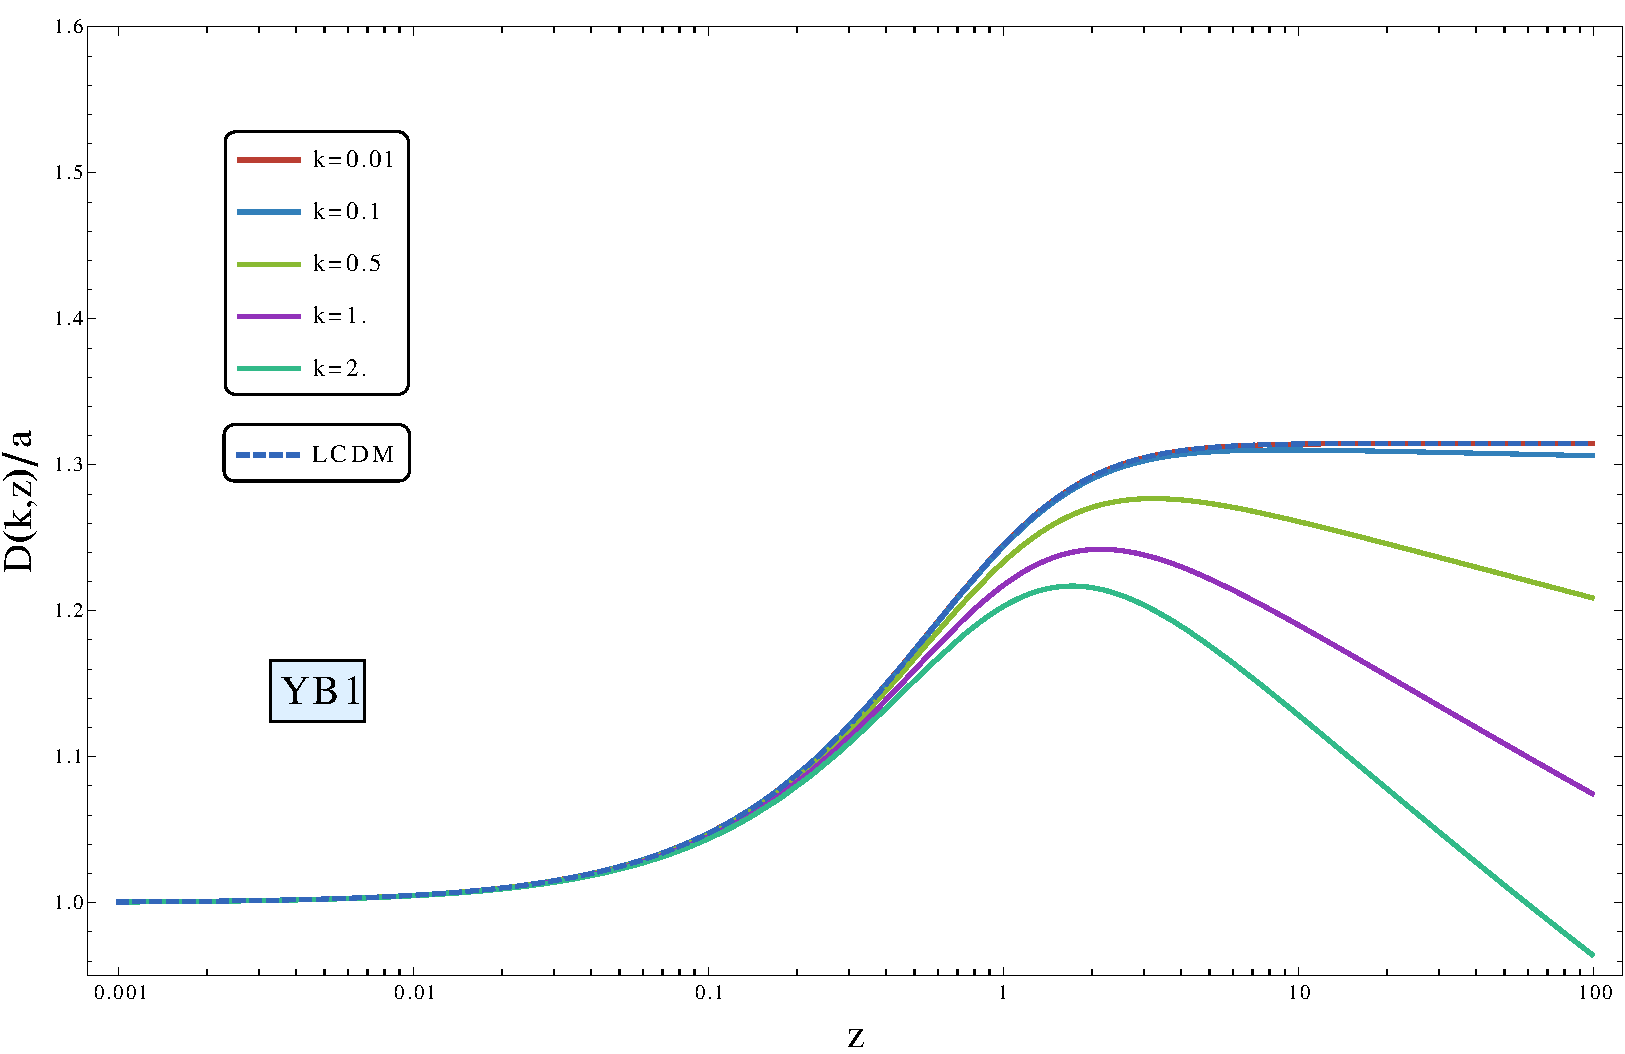
\includegraphics[width=0.7\linewidth]{Chapters/resummation-plots/Dgrowth-YB1}
	\caption[Growth factor in Horndeski.]{Comparison between the growth factor $D_{+}(z,k)$ in a Horndeski model at different
	scales $k$ to the one in the $\lcdm$ case, with equal cosmological parameters. In this model, for non-linear scales $k \gtrsim 0.1$, the growth 
is suppressed at high redshifts $z\gtrsim 1$.}
	\label{fig:change-Dplus-Y}
\end{figure}
For the same model, we can compare how the $f \sigma_{8}$ curve would behave if we include linear or non-linear calculations. This is
shown in \cref{fig:YB1-fsigma8}, where we are using the data points from \mcite{Macaulay et al. (2013)}.
The solid red and blue lines, stand for a linear calculation of $f \sigma_{8}$ at $k=0.01 \mathrm{h/Mpc}$ and 
$k=0.2 \mathrm{h/Mpc}$, respectively. The green line with dots, is a non-linear calculation at  $k=0.01 \mathrm{h/Mpc}$.
We see that the inclusion of non-linearities can play an important role. This simplified Horndeski model, would be still compatible
with the data points shown in red.
\begin{figure}[tbph]
	\centering
	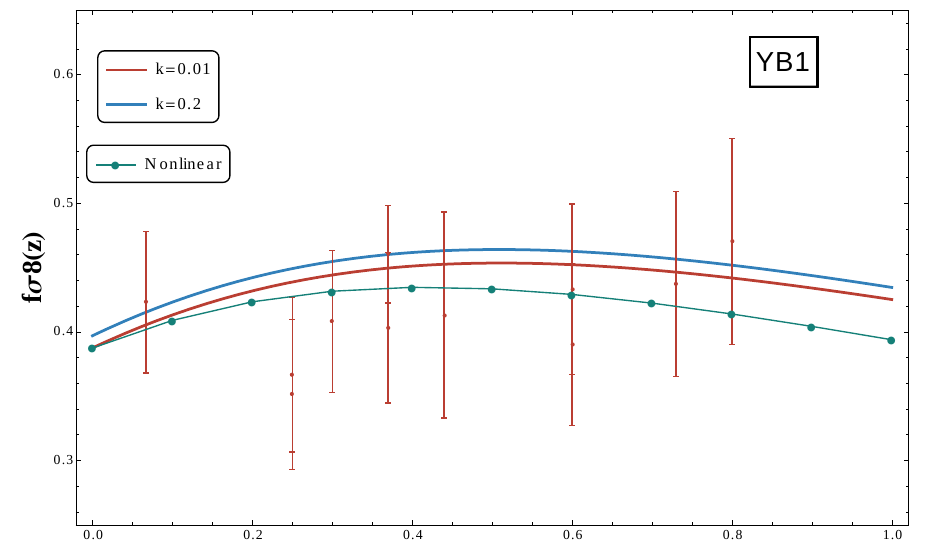
\includegraphics[width=0.7\linewidth]{Chapters/resummation-plots/fsigma8plot-preliminary-YB1.png}
	\caption[$f \sigma_{8}$ in Horndeski.]{For a simple Horndeski model $YB1$,
		 we show the $f \sigma_{8}$ in three different cases. The solid red and blue lines, stand for a linear calculation of $f \sigma_{8}$ 
		 at $k=0.01 \mathrm{h/Mpc}$ and 
		$k=0.2 \mathrm{h/Mpc}$, respectively. The green line with dots, is a non-linear calculation at  $k=0.01 \mathrm{h/Mpc}$. The red data points,
	are taken from \mcite{Macaulay et al. (2013)}.}
	\label{fig:change-fsigma8-Y}
\end{figure}

Finally, we show in \cref{fig:PS-resummed-YB1}, for the same Horndeski model YB1, its non-linear power spectrum vs. the one in $\lcdm$,
with the same cosmological parameters. As a reference, we also show the input linear power spectrum, extrapolated to $z=0$,
using linear theory. We can see that the model YB1 (blue line), has a 1\%
higher power spectrum at scales $k \approx 0.1$, compared to $\lcdm$, increasing up to 5\% at $k \gtrapprox 0.5$.
As we have seen in previous discussions in this dissertation (see \cref{chap:lin-nonlin-MG-forecasts} and \cref{chap:Fitting-CDE}), this is an effect that can be measured by future galaxy redshift surveys.

\begin{figure}[tbph]
	\centering
	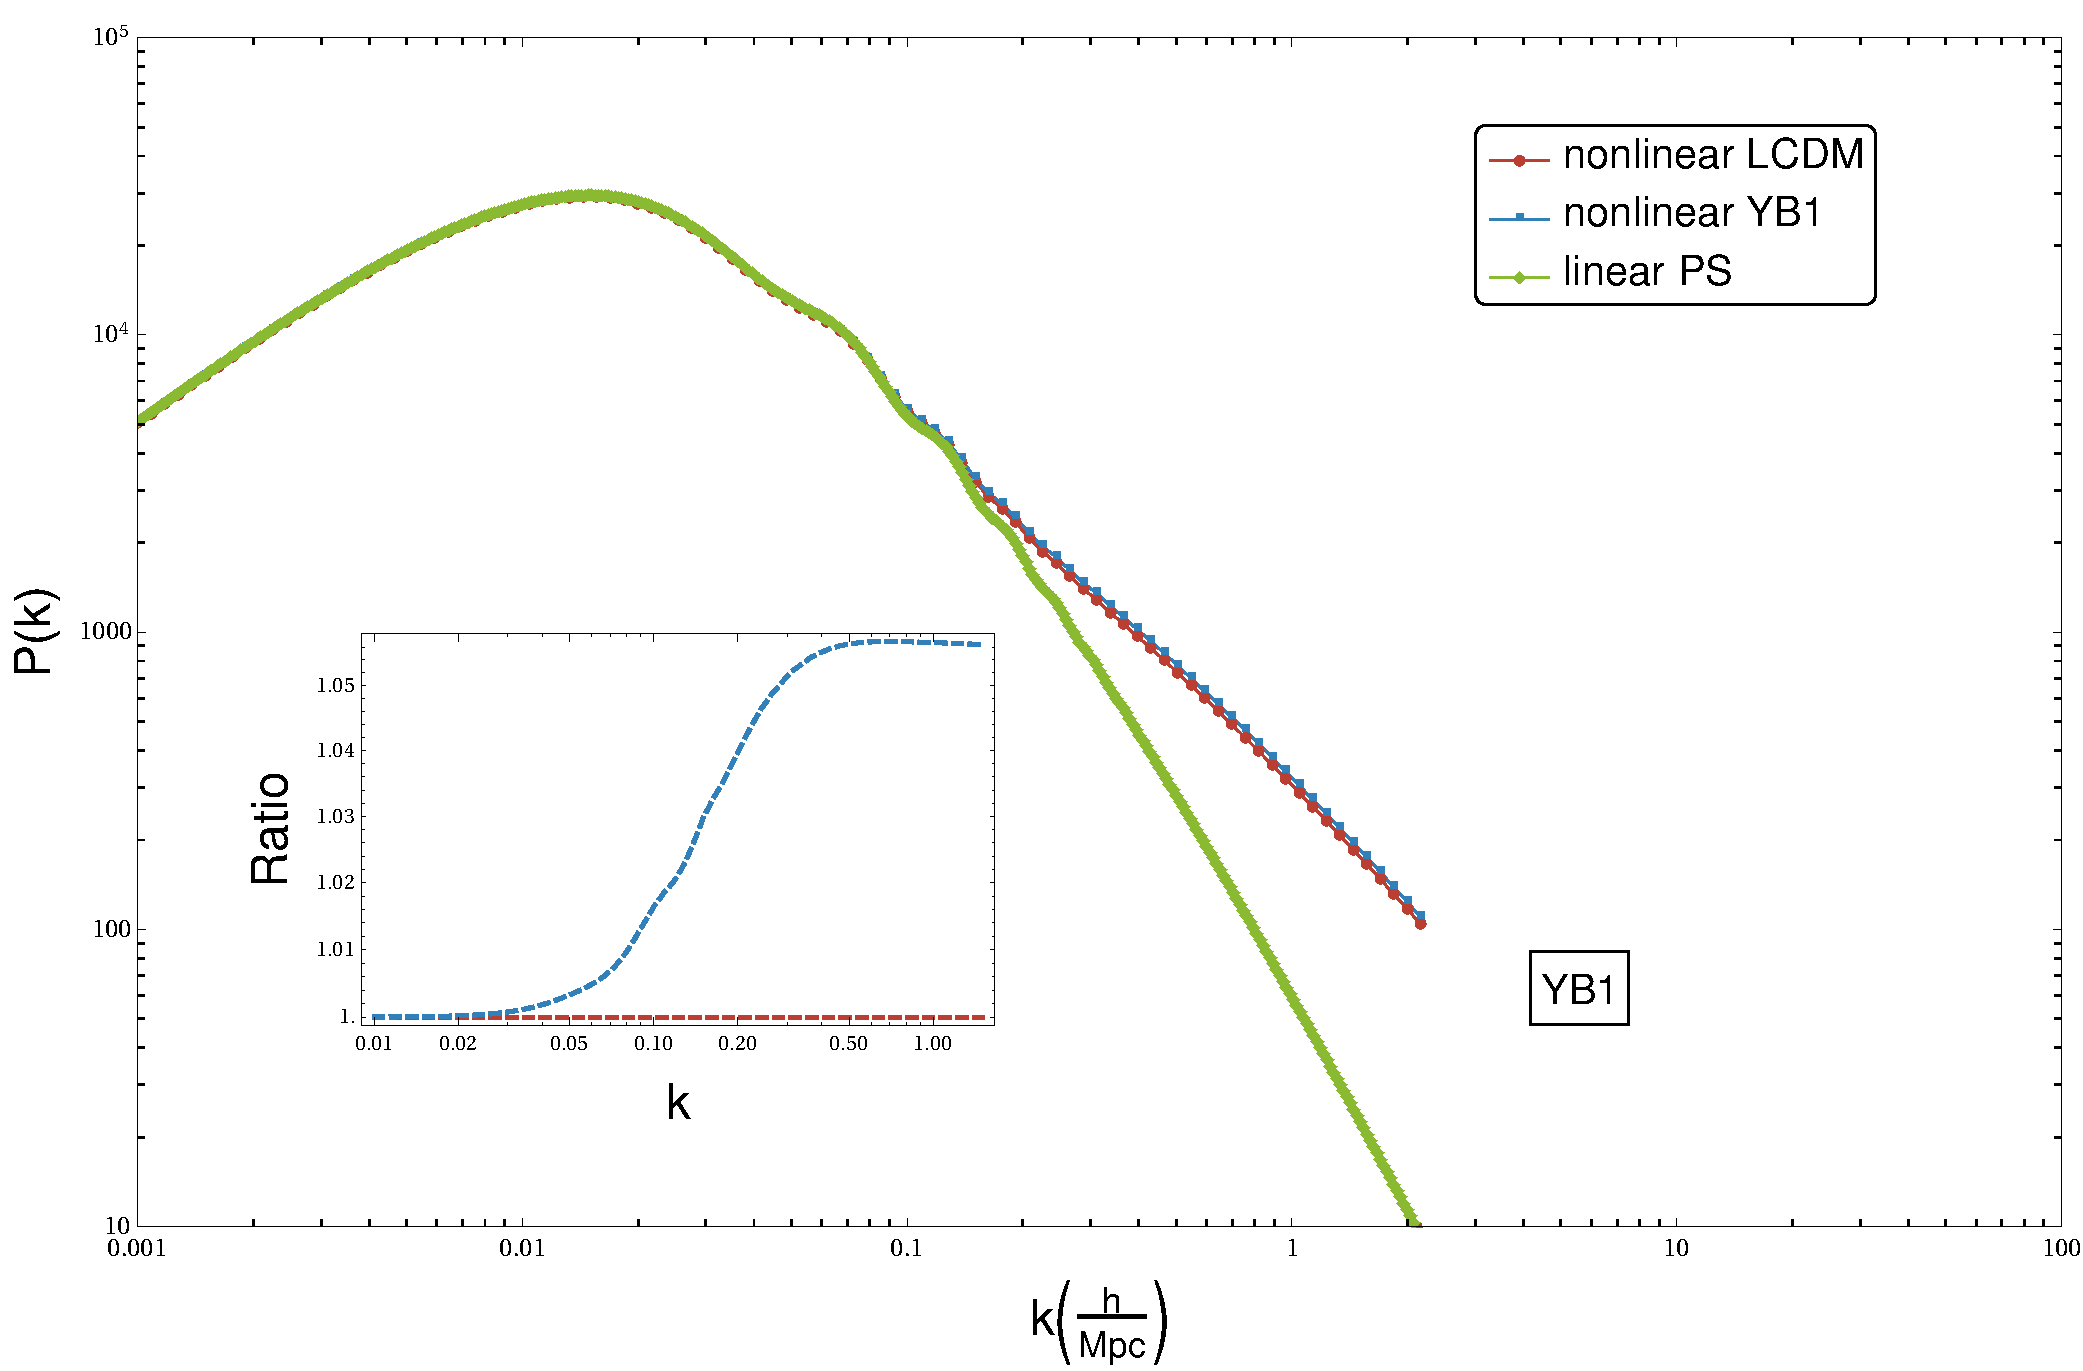
\includegraphics[width=0.9\linewidth]{Chapters/resummation-plots/PS-Resummation-YB1-vs-LCDM.pdf}
	\caption[$f \sigma_{8}$ in Horndeski.]{For the simple model Horndeski model, YB1,
		we show its non-linear power spectrum (blue lines) $P(k)$, compared to the $\lcdm$ case (red lines), with the same parameters.
		The green thick line is the linear input power spectrum. The ratio to $\lcdm$ is shown in the inside box, where the red line is $\lcdm$ and therefore
		equal to 1, while the blue line is the model YB1. The maximum difference to $\lcdm$ is of the order of 5\% at scales $k \gtrapprox 0.5$.}
	\label{fig:PS-resummed-YB1}
\end{figure}

\section{Summary}

In this chapter we have shown first of all how to obtain the linear and non-linear equations
governing the density perturbations of a Cold Dark Matter (and therefore, non-relativistic) component, 
under the influence of gravity.

For the linear theory, we have shown in \cref{sec:DM-growth} that there are several
ways to tackle the problem and that the growth of perturbations can be even solved analytically, see
\cref{eq:Dplus-Hyper}.

For the non-linear theory, we have shown that the full set of fluid equations complicates considerably.
As we have seen, there has been a tremendous progress in the treatment of these equations in the last 10 years and many different
and complimentary techniques have been developed.

Here we chose a specific resummation technique called eikonal Renormalized Perturbation Theory (eRPT, see \cite{anselmi_nonlinear_2012} and
\mcite{Peloso, Pietroni, 2016}) and we applied it for the first time 
to Horndeski models of modified gravity within the quasistatic approximation.
We have been able to compute the linear propagator and the 1-loop integrals in a specific case and we have 
produced the first numerical results. As already stated in the introduction, this is work in progress and the results
still have to be confirmed and checked against N-body simulations and other semi-analytic methods.
In recent years there has been substantial progress in this direction, with more N-body simulations and semi-analytic
methods, capable of calculating structure formation in modified gravity theories (see, \mcite{Winther, Baldi, COLA 2016, Li}).
Moreover, we will also profit from recent Boltzmann codes like \textsc{EFTCAMB} by \cite{hu_eftcamb/eftcosmomc:_2014-1} and 
\textsc{hi-CLASS} by \cite{zumalacarregui} that can provide a more exact initial power spectrum in the models
we are studying here.

The results of this chapter so far, will be published in a paper together with Dr. Massimo Pietroni and
Dr. Valeria Pettorino.





%\section{Numerical approaches}
%
%\subsection{N-body simulations}
%\begin{itemize}
%\item The Vlasov-Poisson system can be discretized on a grid and the denisty
%can be represented with particles
%\item Particle-Mesh method
%\item Tree method
%\item Extraction of information: The power spectrum and Halo catalogs
%\end{itemize}
%
%
%
%As we have seen in the previous chapters, non-linear dynamics of gravitational
%interactions, are hard to treat analytically. If we want to study
%the growth of perturbations in the full non-linear regime, as well
%as in large scales and at galactic scales, we need to perform numerical
%simulations. Numerical N-body simulations have many advantages, as
%well as some drawbacks related to their specific practical implementation
%and we will try to explain here only some of their most fundamental
%properties. 
%
%%In this work we are using the CoDECS simulations, which are a modification
%%of the parallel Tree-PM N-body code of GADGET-2 (see \citet{baldi_hydrodynamical_2008,baldi_codecs_2011}).
%%In order to understand what this means and what its properties and
%%parameters are, it is necessary to explain some technical issues regarding
%%the computational techniques of current cosmological simulations.
%
%First we will review some general techniques to deal with great numbers
%of particles in gravitational interactions, then we will review some
%of the most important Dark Universe simulations and finally we will
%explain some technicalities regarding the extraction of the power
%spectrum from simulation data. 


\section{Excursion into other computational techniques: N-body simulations \label{sec:Computational}}


As we have seen repeatedly in the previous chapters, non-linear structure formation 
is of extreme importance for the era of precision cosmology.
In order to connect our analytic and semi-analytic methods presented in \cref{chap:lin-nonlin-MG-forecasts}
and \cref{chap:nonlinear} with a fully non-linear N-body treatment discussed in \cref{chap:GNQ} below,
we will review in this section some of the fundamental properties of N-body simulations.

The progress in this field has been impressive and nowadays N-body codes are capable
of simulating trillions of particles \mcite{Illustris, Coyote, DEUS}, including not only 
gravitational physics, but also star formation, galactic and supernova feedback, magnetic fields and
many more complicated astrophysical phenomena \mcite{Illustris, Springel}.

To perform an exact evolution of the density fluctuations, beyond
linear perturbations, the density field has to be represented by a
set of fictitious discrete particles with a certain mass. These particles
do not represent real galaxies or clusters of galaxies, they just
sample the underlying density field. For current cosmological simulations,
depending on the desired resolutions, the particle masses are around
$m_{p}\approx10^{9}-10^{12}M_{\odot}$, see \citet{kuhlen_numerical_2012}.
\footnote{Parts of the following text have appeared as part of papers by the author (see list of papers)
and as part of his Master thesis, presented at the University of Heidelberg, 2013.}

The equations of motion for each particle depend on solving for the
gravitational field due to all the other particles, finding the change
in particle positions and velocities over some small time step. Then
particle positions and velocities have to be updated and the gravitational
potentials have to be recalculated to start a new iteration. For cosmological
simulations, where we suppose the Universe to be isotropic and homogeneous
at large scales and described by a smooth FLRW metric, we use the
fact that at smaller scales the Universe must tend to locally inertial
frames where Newton's laws are valid. Therefore we can just use Newtonian
dynamics and the expansion history of the Universe is taken into account
by using comoving coordinates, where the expansion rate $a(t)$ is
factored out (see \citet{peacock_cosmological_1999,dehnen_n-body_2011}).
We then obtain for the comoving velocity $u$ the following equations:
\begin{equation}
\frac{d}{dt}\vec{u}=-2\frac{\dot{a}}{a}u-\frac{1}{a^{2}}\nabla\Phi
\end{equation}
where $\Phi$ is the Newtonian gravitational potential due to density
perturbations. If we change the time variable from $t$ to $a$ we
obtain:
\begin{equation}
\frac{d}{d\mbox{ln}a}(a^{2}\vec{u})=\frac{a}{H}\vec{g}=\frac{G}{aH}\sum_{i}m_{i}\frac{\vec{x_{i}}-\vec{x}}{\left|\vec{x_{i}}-\vec{x}\right|^{3}}
\end{equation}
We see that in order to get the gravitational acceleration for one
single particle, we have to sum the contributions from all other particles,
which leads to the exact solution, but it is computationally prohibitive
for a large number of particles, since the number of needed computations
grows as $\mathcal{O}(N^{2})$. 

Since we have only finite resources for computation, we need to calculate
the particles in a finite box of size $L$ and a finite number of
particles $N$. In this case the walls of the box would break our
desired homogeneity and isotropy, therefore we need to introduce periodic
boundary conditions, such that the cubic box is actually a 3-torus,
where the walls on opposite sides are identified. Then the gravitational
potential can be described as (\citet{dehnen_n-body_2011}): 
\begin{equation}
\Phi(\mathbf{x},t)=-G\sum_{\mathbf{n}}\int d\mathbf{x}'\,\frac{\rho(\mathbf{x}'+\mathbf{n}L,t)}{\left|\mathbf{x-x}'-\mathbf{n}L\right|}
\end{equation}
where the sum is performed over $\mathbf{n}=(N_{x},\,N_{y},\,N_{z})$
and accounts for all periodic replica. Usually all the $N_{i}$ are
the same in all directions. Because of the fact, that performing an
infinite sum of replicas is in practice not possible, the sum is approximated
using Ewald's method (see \citet{ewald_berechnung_1921}), which was
originally developed for periodic crystals in solid state physics
and was first adapted to this field by \citet{hernquist_application_1991}.

The gravitational Newtonian force has a singularity when two particles
approach too close to each other, that is why a so-called softening
term has to be added to the force equation in order to avoid unphysical
accelerations during close encounters. The force can be modified for
small distances to something like (see \citet{trenti_gravitational_2008}):
\begin{equation}
\vec{F_{i}}=-\sum_{j\neq i}Gm_{i}m_{j}\frac{\vec{x_{i}}-\vec{x_{j}}}{\left(\left|\vec{x_{i}}-\vec{x_{j}}\right|^{2}+\epsilon^{2}\right)^{3/2}}
\end{equation}
where $\epsilon>0$ is the softening or smoothing length, which is
a typical size below which the gravitational interaction is suppressed.
In current cosmological N-body simulations, the softening length is
found to be: $1.0h^{-1}\mbox{kpc}\leq\epsilon\leq150h^{-1}\mbox{kpc}$,
meaning that most of the simulations cannot resolve halos or subhalos
of galaxies and can only focus on large scale structure formation.
The choice of gravitational softening length is still a debate among
the community, since making it to small increases computational effort
(due to smaller time steps), but allows for more realistic gravitational
potentials and on the other hand it introduces spurious two-body relaxation
effects that can cause artificial fragmentation of structure (see
\citet{kuhlen_numerical_2012} and references therein).

Many alternatives to direct summation of forces, have been developed
in the last 20 years, also using hybrid approaches. The most relevant
ones for our purposes are the following (see reviews by \citet{trenti_gravitational_2008,dehnen_n-body_2011,kuhlen_numerical_2012}):
\begin{itemize}
\item \textbf{Particle Mesh PM: }Since the problem is to solve Poisson's
equation, a faster approach is to use Fourier methods for discretized
systems, such as the FFT (see \ref{sub:Fourier-Transform-Discr})
 and solve directly for Poisson's equation in Fourier space: 
\begin{equation}
(\nabla\Phi)_{k}=-i\Phi_{k}\mathbf{k}=\frac{-i4\pi Ga^{2}\overline{\rho}}{k^{2}}\delta_{k}\mathbf{k}
\end{equation}
Then we can eliminate the matter density in terms of $\Omega_{m}$
and for a given particle, the equation of motion would be: 
\begin{equation}
\frac{d}{d\mbox{ln}a}(a^{2}\mathbf{u})=\sum\mathbf{F}_{k}\mbox{exp}(-i\mathbf{k}\cdot\mathbf{x}),\qquad\mathbf{F}_{k}=-i\mathbf{k}\frac{\Omega_{m}Ha^{2}}{2k^{2}}\delta_{k}
\end{equation}
By interpolating the density field $\rho_{k}$ over a finite grid,
one can solve Poisson's equation and then use the FFT again to calculate
the forces and velocities on the particles. The complicated part of
the algorithm is the assignement of the mass of the particles onto
the grid cells and then interpolating back the evaluated force onto
the particles, for consistency the same procedure has to be used for
both these steps. Particles do not interact with each other but only
through the mean field, which causes that the maximum force resolution
to be limited to about the size of the mesh. The computational advantage
of this method is that the number of computations is now of the order
$\mathcal{O}(N_{g}log(N_{g}))$, for $N_{g}$ the number of grid cells.
This is the scaling of the FFT method also (see \ref{sub:Fourier-Transform-Discr}).
\item \textbf{Particle-particle-particle-mesh $\mathbf{P^{3}M}:$ }Since
PM codes are gravitationally softened below the mesh size and the
resolution is therefore low, this hybrid method uses a coarse grid
to calculate forces at larger scales between distant cells and for
particles in the same or neighbouring cell, a direct sumation between
particles is performed, increasing the force resolution, but also
in some way the computational time, if there is a strong clustering
of particles.
\item \textbf{Adaptive Mesh Refinement AMR: }The dynamic range of particle-mesh
codes can be increased by using instead of a static grid, an adaptive
one, which has more concentrated grid elements in the high density
regions, where the forces are also more varying and stronger. This
allows to truncate the error to the desired precision level by refining
the mesh at specific points. The complicated part of this method is
to match the solution at the grid interfaces, where they might change
drastically. Since the force softening can change along a particle's
orbit, this method can lead to an unphysical violation of energy conservation.
To accelerate the calculation of an AMR code, one can evolve the particles
asynchronously, leaving the particles in the coarse grid, while evolving
with smaller time steps the ones in the finer grid and using the coarser
grid potential as a boundary condition.
\item \textbf{Tree Codes: }If close encounters are not important and the
force contributions from distant particles do not have to be calculated
at high accuracy, this method is well suited for cosmological simulations.
The simulation box is split into eight cubic cells, containing a determined
number of particles, each cubic cell containing fewer than $n_{max}$
number of particles is split again into eight cubic child cells of
half their parent's particle size. This results in a tree-like binary
(oct) hierarchy of cubic nodes, containing the root box (that contains
all $N$ particles) at his bottom. For each cubic cell, the total
mass and center of mass is calculated and stored as an information
on the node. Then at the moment of calculating the force acting on
a particle at position $\vec{x}$, one just adds the contributions
from different cells with center of mass $\vec{z_{a}}$, depending
on some opening angle: $\mbox{sin}(\theta)=\left|\vec{x}-\vec{z}_{a}\right|/w_{a}$,
where $w_{a}$ is the linear size of the box (this is the easiest
approximation, for a formal derivation of the tree code, using taylor
expansions and multipoles, see \citet{dehnen_n-body_2011}). If the
opening angle is bigger than wanted, one applies the algorithm to
the daughter cells. In this way one gets the contributions from all
possible groups of particles. This method offers a computational time
that scales like the depth of the tree, therefore being of order $\mathcal{O}(N\mbox{ln}(N))$,
which is similar to the above mentioned methods. For nearby particles,
a standard particle-particle interaction is calculated. The complicated
aspect of the tree method is, among others, how to visit each cell
only once, in a highly parallelizable way. Really efficient methods
have been developed, using Peano-Hilbert curves, such as in the Gadget-2
code, which is a Tree-PM code (\citet{springel_cosmological_2005}).
A drawback of this method is that each interaction is only one-sided,
meaning that the force of a single particle on the group of particles
of a distant cell is not calculated and therefore Newton's third law
is violated. This can lead to fluctuations in the total energy of
the N-body system, but it has been shows that this spurious effects
can be kept quite small (see \citet{dehnen_n-body_2011}). In \ref{fig:5.1}
(top), the binary tree hierarchy of the simulation box can be seen
and (bottom) a comparison between the computation of the force with
direct sumation and the tree algorithm. The computational advantage
of the tree algorithm can be really appreciated in this case.
\item \textbf{Fast Multipole Methods FMM: }This modern method uses the fact
that in a standard tree implementation, one does not take advantage
of the fact that the force caused by distant cells will be the same
for nearby particles. This method not only expands the distant source
potentials into multipoles, but also expands the force at the sink
position, leading to a gain in speed that is quite considerable, leading
to computational efforts of order $\mathcal{O}(N)$. Since the interaction
is approximated by cells at both ends of the interaction (each interaction
is mutual), Newton's third law is respected and no spurious effects
arise. At nearby distances a particle-particle method is employed
as usual. The drawback of this method is that its parallelization
is not so straighforward and has not been developed yet. For more
references, check \citet{dehnen_n-body_2011}.
\end{itemize}

%\begin{figure}[h]
%%\parbox[t]{1\columnwidth}{%
%%\noindent \begin{center}
%%\includegraphics[width=0.9\textwidth]{Figures/SpringelOctTree}
%%\par\end{center}%
%%}\vspace{0cm}
%%
%%
%%\parbox[t]{1\columnwidth}{%
%%\noindent \begin{center}
%%\includegraphics[width=0.9\textwidth]{Figures/TreeMethod}
%%\par\end{center}%
%\caption[\textbf{Top}: Hierarchical structure of a Tree code, the fundamental
%box is divided into always smaller cells. Figure taken from: \citet{springel_cosmological_2005}.
%\textbf{Bottom}:Comparison between force calculation for 100 particles.
%Figure taken from: \citet{dehnen_n-body_2011}.]{\label{fig:5.1}\textbf{Top}: Hierarchical structure of a Tree code,
%the fundamental box is divided into always smaller cells. A Peano-Hilbert
%curve method (space filling curve) is used to visit all cells in parallel.
%Figure taken from: \citet{springel_cosmological_2005}. \textbf{Bottom}:
%Comparison between force calculation for 100 particles. Left: Each
%red curve represents a direct particle-particle interaction. Middle:
%The tree method, with its cells and groups of particles (green lines
%represent particle-cells interactions). Only 7 interactions are needed
%to compute total force. Right: Interactions needed to compute all
%the forces among particles, requiring 902 cell-particle interactions
%and 306 particle-particle interactions, instead of 4950 computations
%in the case of the direct summation. Figure taken from: \citet{dehnen_n-body_2011}.}
%\end{figure}


%\subsection{Fitting formulae and prescriptions}
